\documentclass[a4paper,twoside,flushend, 10pt]{article}
\usepackage{times}
\usepackage{ijfis-scopus}
\usepackage{color}
\usepackage{epsfig, picins, graphicx}
\usepackage{paralist}
\usepackage{cite}
\usepackage{amsmath,amssymb,amsfonts,mathtools}
\usepackage{algorithmic}
\usepackage{textcomp}
\usepackage{xcolor}
\usepackage{amsthm}
\usepackage{mathabx}
\usepackage{hyperref}
\usepackage{caption}
\usepackage{tablefootnote}
\usepackage{array}
\usepackage{mathrsfs}
\usepackage{kotex}
\usepackage{float}
\usepackage{multirow}
\usepackage{colortbl}
\usepackage{booktabs}
\usepackage{xcolor}

\usepackage{xpatch}

%===========================================================

\begin{document}



\title{Application of TimeGPT for enhancing water level prediction in Gamcheon River, Korea}

%%
\author{Jon-Lark Kim\inst{1}\inst{2}, Jae-Hyun Baek\inst{1}\inst{2}, Keon-Hwi Kim\inst{1}\inst{2}, Tae Hyo Baek\inst{3} and Chang-Lae Jang\inst{3}}

\institute{
Department of Mathematics, Sogang University, Seoul, Korea
\and
Institute for Mathematical and Data Sciences, Sogang University, Seoul, Korea
\and
Department of Civil Engineering, Korea National University of Transportation, Chungju-si, Korea
}

\begin{abstract}
This study is the first attempt to predict the water level of the Gamcheon River, Korea, using the LLM-based TimeGPT. Our research showed that TimeGPT performed better than existing time series models including SARIMAX and DLinear. TimeGPT provided better prediction accuracy for short-term and long-term forecasts under Nash-Sutcliffe Efficiency scores. TimeGPT effectively captured water level changes by integrating rainfall data. Our approach will offer insights for water resource management and flood prediction.
\end{abstract}

\begin{keyword}
Water-level prediction, time series analysis, LLM-based methods
\end{keyword}

\maketitle
\runningtitle{2025}{}{}{}{}{Jon-Lark Kim, Jae-Hyun Baek, Keon-Hwi Kim, Tae Hyo Baek and Chang-Lae Jang}{}
\makefoot{}{}{}{Jon-Lark Kim and Chang-Lae Jang}{jlkim@sogang.ac.kr and cljang@ut.ac.kr}{8}\hspace{0.5cm}
\begin{minipage}[t]{13cm}
%===========================================================
\section{Introduction}
\noindent

Accurate prediction of water levels is a critical component in managing river systems. This study focuses on the Gamcheon River in Gyeongsangbuk-do, a 69\,km tributary of the Nakdong River with a 1{,}022.13\,km$^2$ basin that flows northeast through Gimcheon-si and Gumi-si. The river’s upper catchment includes the \textit{Gimcheon--Buhang Dam}, a multi-purpose concrete-faced rockfill dam (CFRD) located on the Buhang Stream in Yuchon-ri, Buhang-myeon, Gimcheon-si. The Gamcheon watershed is characterized by a wide and shallow channel with significant bed variability, making hydrological prediction particularly challenging. Figure~\ref{fig:seonjugyo} illustrates the major observation stations, including Seonjugyo, a key checkpoint for water-level monitoring.

\begin{figure}[H]
    \centering
    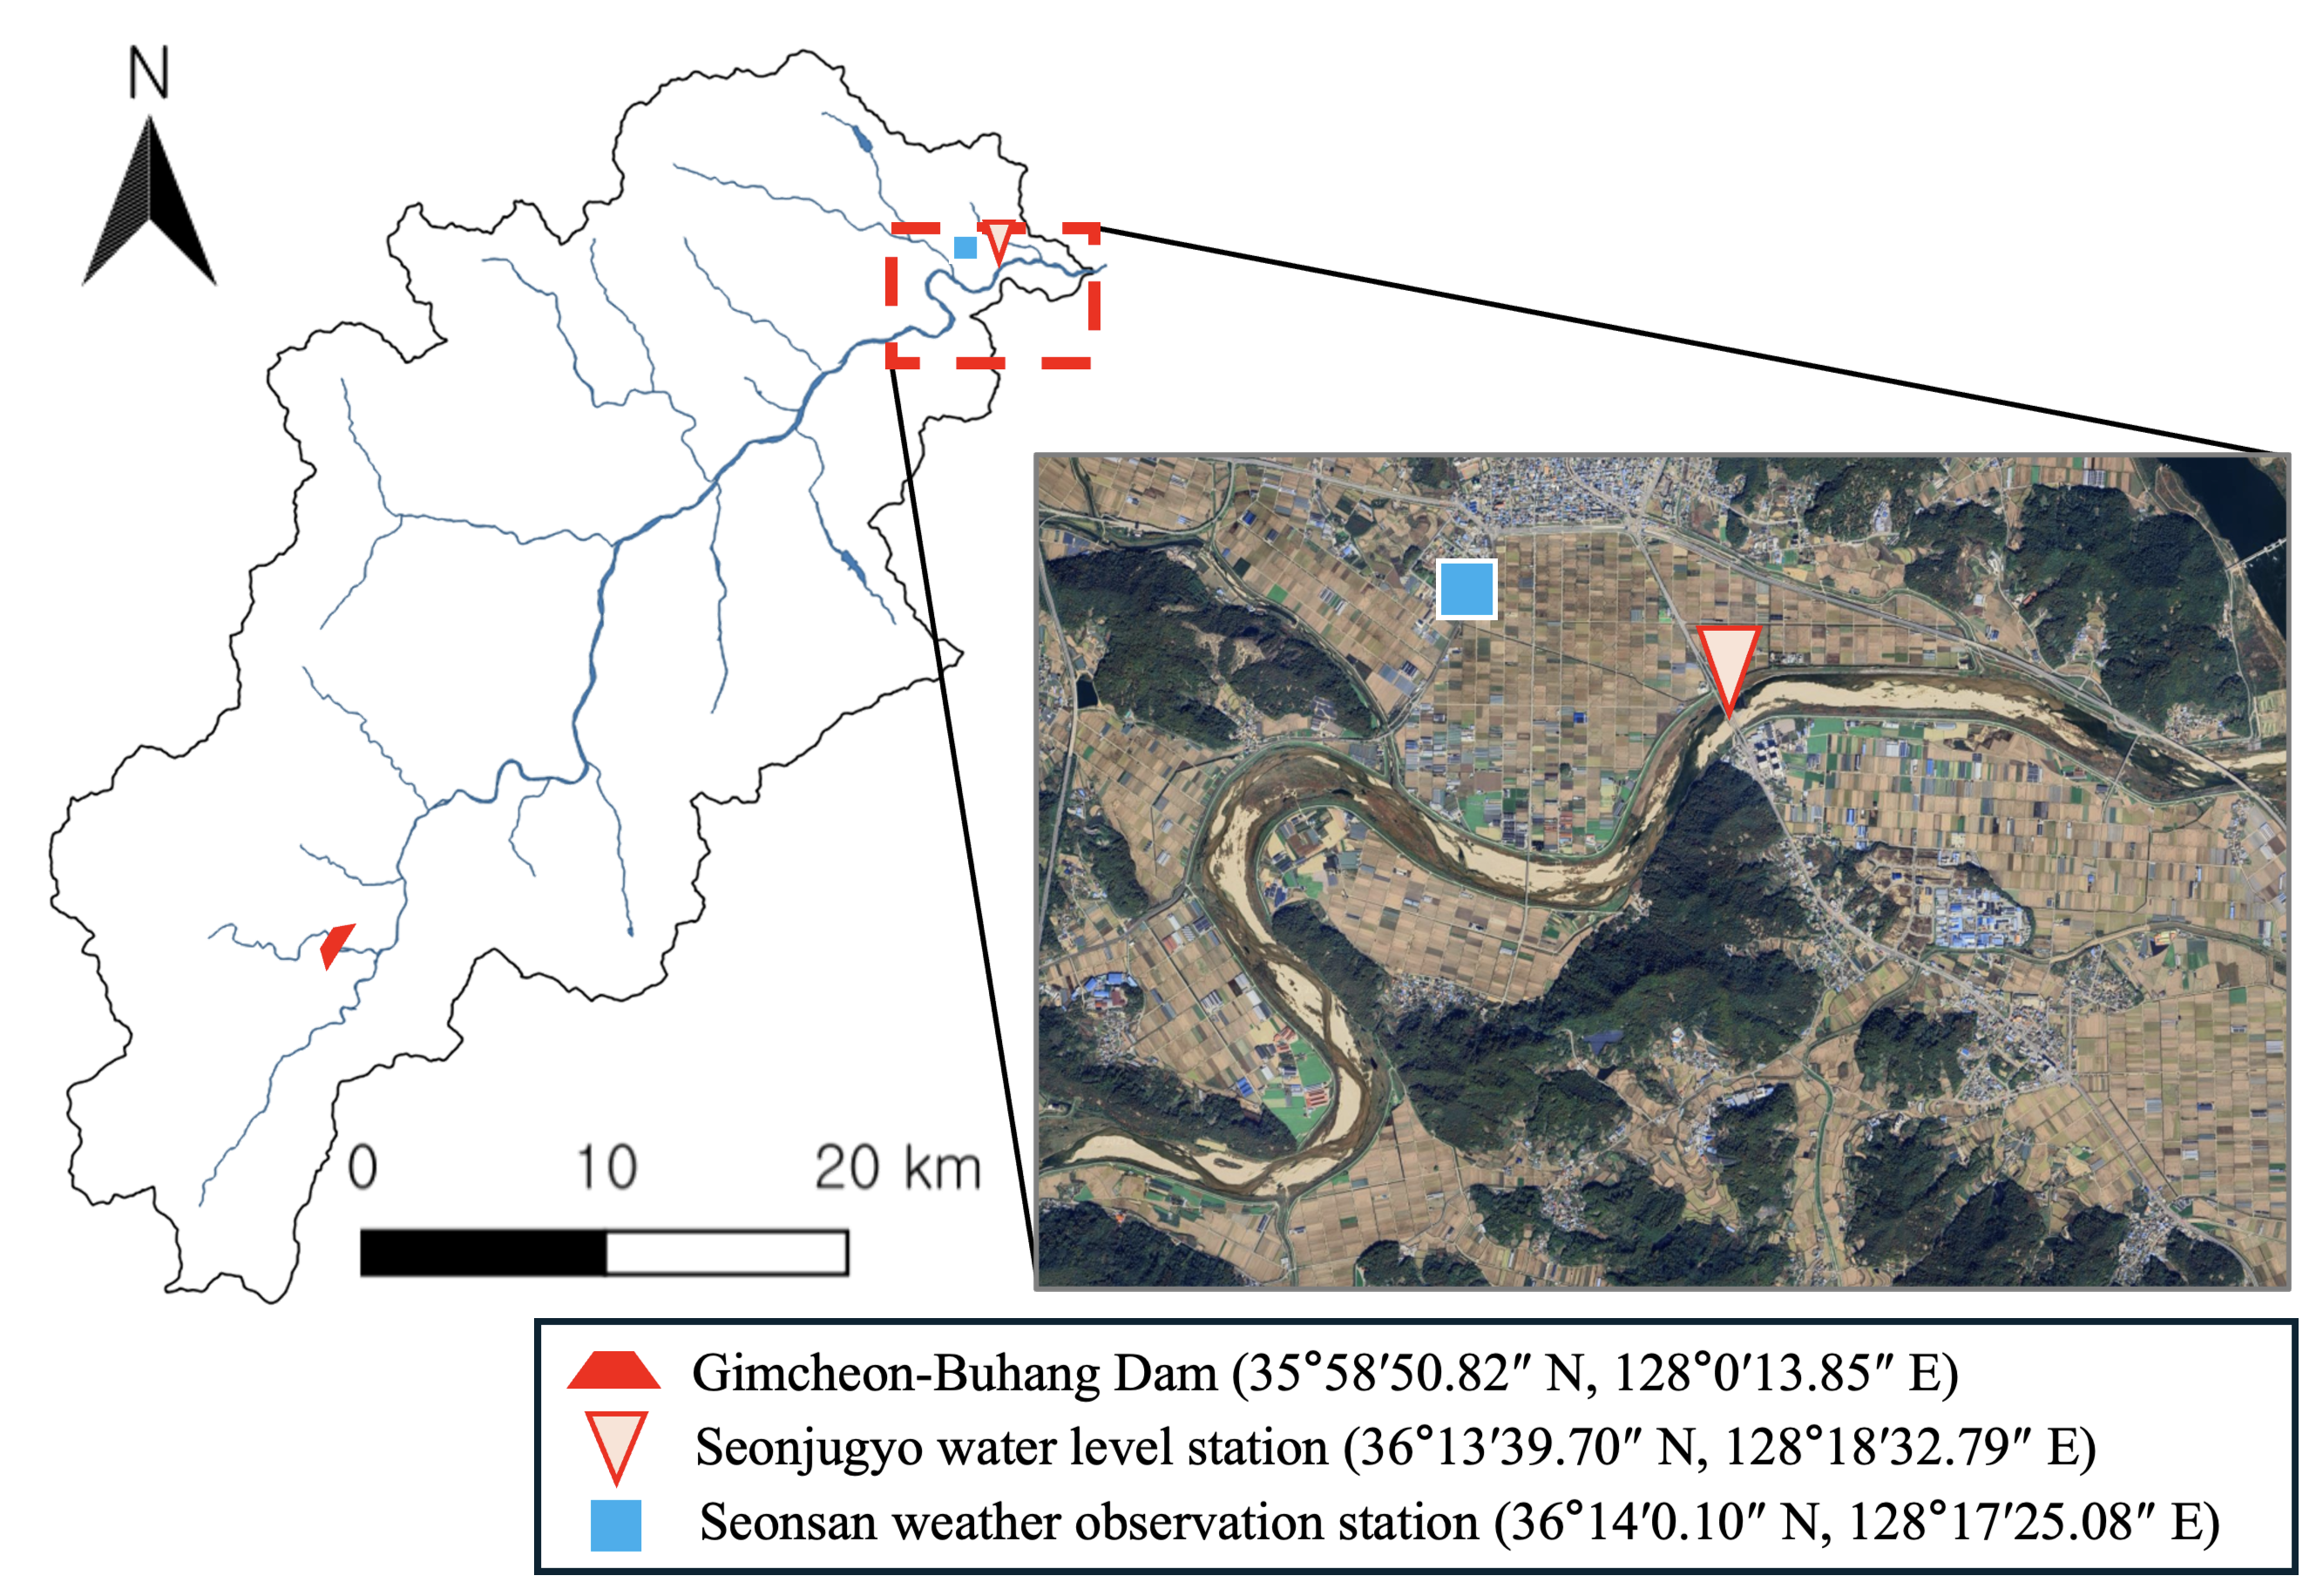
\includegraphics[width=85mm]{gamcheon_overview.png}
    \vskip -0.5pc
    \caption{Major observation stations and dam locations in the Gamcheon watershed.}
    \label{fig:seonjugyo}
\end{figure}

\end{minipage}
\newpage

While the dam plays an essential role in flood control and stable water supply, scheduled discharges can cause sudden changes in downstream water levels independent of rainfall \cite{KCP2023, YY24}. Coupled with the Gamcheon’s sensitivity to summer monsoons and historical floods during Typhoons Rusa (2002) and Maemi (2003), these factors highlight the need for forecasting systems capable of addressing both natural and operational hydrological drivers. In recognition of these challenges, the Korea Ministry of Environment, through the Korea Environmental Industry \& Technology Institute (KEITI), designated the Gamcheon basin as a test bed for the project “Research and Development on the Technology for Securing Water Resources Stability in Response to Future Change.”

Recent advancements in machine learning, particularly deep learning approaches such as LSTM \cite{HS1997} and Transformer architectures \cite{VSP17}, have shown promising results in time series forecasting tasks. These models excel at capturing complex temporal patterns, especially for extended horizons, as demonstrated in related environmental studies \cite{XFL23}. However, they face notable challenges: high computational cost and careful calibration for environmental data with missing values, irregular sampling, and sudden weather- or operation-induced shifts. Traditional statistical approaches like ARIMA and SARIMAX \cite{BJ2015} remain interpretable and simple, yet often struggle to fully capture these complexities, motivating more advanced solutions.

Our contributions are threefold. (1) We conduct the first comprehensive application of diverse forecasting models to the Gamcheon River dataset; (2) we provide a detailed comparative analysis highlighting the strengths and limitations of classical, linear, and LLM-based models in addressing the challenges of environmental time series forecasting; and (3) as far as we know, this is the first study to apply TimeGPT and its enhanced version with external variables to water level forecasting, demonstrating significant improvements in prediction accuracy across different temporal horizons.

By employing a scenario-based approach, we offer a layered understanding of how different forecasting models perform under varying levels of complexity and how they can be effectively integrated to enhance forecasting accuracy. Our study sets a precedent for future research in environmental forecasting, emphasizing the importance of leveraging both traditional and modern machine learning techniques to tackle real-world challenges.

The remainder of this paper is organized as follows. Section 2 provides a comprehensive review of the literature on time series forecasting, from classical statistical methods to recent LLM-based approaches. Section 3 introduces the preliminary concepts and models used in our study, including the limitations of transformer-based models and the architectures of Linear models and TimeGPT. Section 4 details our experimental setup, outlining the novel implementation on the Gamcheon dataset and the scenario-based comparative analysis. In Section 5, we present and analyze the results from our three scenarios. Finally, Section 6 concludes the paper with a summary of our findings and their implications for future research in water resource management.

\section{Literature review}
\noindent
The field of time series forecasting has witnessed significant advancements in recent years, particularly with the emergence of foundation models and large language models (LLMs). A comprehensive review of the literature reveals several key developments that have shaped our current understanding and approaches to time series analysis.

Early work in time series forecasting primarily focused on statistical methods, as evidenced by the seminal works of Box and Jenkins \cite{BJ1970} and their subsequent refinements \cite{BJ2015}. These classical approaches laid the groundwork for understanding temporal dependencies and seasonal patterns in time series data. The introduction of SARIMAX models \cite{HK2008} and later the Prophet framework \cite{TL2018} represented significant steps forward in handling complex seasonal patterns and external variables.

A paradigm shift occurred with the advent of deep learning approaches, particularly through the work of Graves and Schmidhuber \cite{GS2005} on Long Short-Term Memory (LSTM) networks. This was followed by transformer-based architectures, which raised important questions about their effectiveness in time series forecasting, as explored by Zeng et al. \cite{ZCLX23}. The evolution continued with specialized architectures like Informer \cite{ZZP2021} and Autoformer \cite{XTZ2021}, which addressed specific challenges in long-sequence time series forecasting.

A significant breakthrough came with the introduction of TimeGPT \cite{GM2023}, a large time series model trained on massive and diverse datasets comprising 100 billion data points across various domains including finance, transportation, banking, web traffic, weather, energy, and healthcare. This innovation represented a departure from traditional approaches by demonstrating that pre-trained models could generate accurate predictions across diverse datasets without additional training. TimeGPT's ability to perform zero-shot inference while maintaining high performance and efficiency has opened new possibilities in the field, suggesting that insights from broader artificial intelligence domains can be effectively applied to time series analysis. As demonstrated by Liao et al. \cite{LWY2025}, TimeGPT exhibits robust performance in scenarios with limited historical data, where it has shown superior predictive capabilities compared to conventional benchmarks, especially for short-term forecasting horizons, achieving significant improvements in both accuracy and computational efficiency.

The development of TIME-LLM by Jin et al. \cite{JWM2024} further expanded on these foundations, demonstrating how large language models, successful in other domains, could be reprogrammed for numerical time series forecasting. Concurrently, recent work has explored the efficiency of such models, with Li et al. \cite{LJX2019} addressing memory bottlenecks in transformer architectures and Liu et al. \cite{LLZ2021} investigating decomposition approaches. These developments in model adaptation and efficiency have contributed to making advanced forecasting methods more practical for real-world applications, particularly in environmental monitoring systems like the Gamcheon water level prediction task.

\section{Preliminaries}

In this section, we present a comparative study of several time series models used to predict water levels at the Seounju-kyo checkpoint. Classical approaches, such as ARIMA, SARIMAX, and Prophet (overview in Table \ref{tab:models_overview}), are utilized as benchmarks to validate the performance of our proposed model.

\begin{table}[H]
    \centering
    \renewcommand{\arraystretch}{1}
    \setlength{\tabcolsep}{8pt}
    \caption{Overview of classical time series models.}
    \label{tab:models_overview}
    \footnotesize
    \begin{tabular}{|>{\columncolor{blue!15}}c|>{\columncolor{yellow!15}}p{5cm}|}
        \hline
        \rowcolor{gray!30}
        \textbf{Model} & \textbf{Details} \\ \hline
        \multirow{3}{*}{\textbf{ARIMA (1970s)}} & Key Features: \newline Non-stationary data handling, autoregressive \\ \cline{2-2}
         & Reference: Box et al. (1970) \cite{BJ1970} \newline Updated reference: Box et al. (2015) \cite{BJ2015} \\ \cline{2-2}
         & Citations: 20,000+ \\ \hline
        \multirow{2}{*}{\textbf{SARIMAX (1990s)}} & Key Features: \newline Seasonal components, exogenous variables \\ \cline{2-2}
         & Reference: Hyndman et al. (2008) \cite{HK2008} \newline Citations: 5,000+ \\ \hline
        \multirow{2}{*}{\textbf{Prophet (2017)}} & Key Features: \newline Trend, seasonality, holidays, missing values \\ \cline{2-2}
         & Reference: Taylor and Letham (2018) \cite{TL2018} \newline Citations: 3,000+ \\ \hline
    \end{tabular}
\end{table}

\subsection{Challenges of traditional transformer-based models}

While Transformer architectures have revolutionized Natural Language Processing (NLP) and Computer Vision (CV), their direct application to time series forecasting has faced scrutiny \cite{ZCLX23}. A primary challenge for standard Transformer models, particularly when trained from scratch on limited datasets, is the permutation-invariant nature of the self-attention mechanism. Without specialized temporal modifications, these models may struggle to preserve the distinct ordering of time-series data as effectively as Recurrent Neural Networks (RNNs) or even simple linear models.

Additionally, standard Transformers are notoriously data-hungry and computationally intensive. The quadratic complexity of the self-attention mechanism ($O(L^2)$) with respect to sequence length $L$ can become a bottleneck for long-term forecasting. Furthermore, when training data is insufficient, these complex models are prone to overfitting, often failing to generalize better than parsimonious statistical methods. This "validity debate" highlights that architectural complexity does not automatically guarantee superior forecasting performance in the absence of massive scale or specialized inductive biases.

\subsection{Linear, DLinear, and NLinear models}

In response to the challenges of complex Transformer architectures, recent research has revisited simpler principles. The LTSF-Linear family of models (Figure \ref{fig:linear}), introduced by Zeng et al. \cite{ZCLX23}, demonstrates that streamlined architectures can often outperform complex Transformers that are not pre-trained at scale.

\begin{figure}[H]
\centering
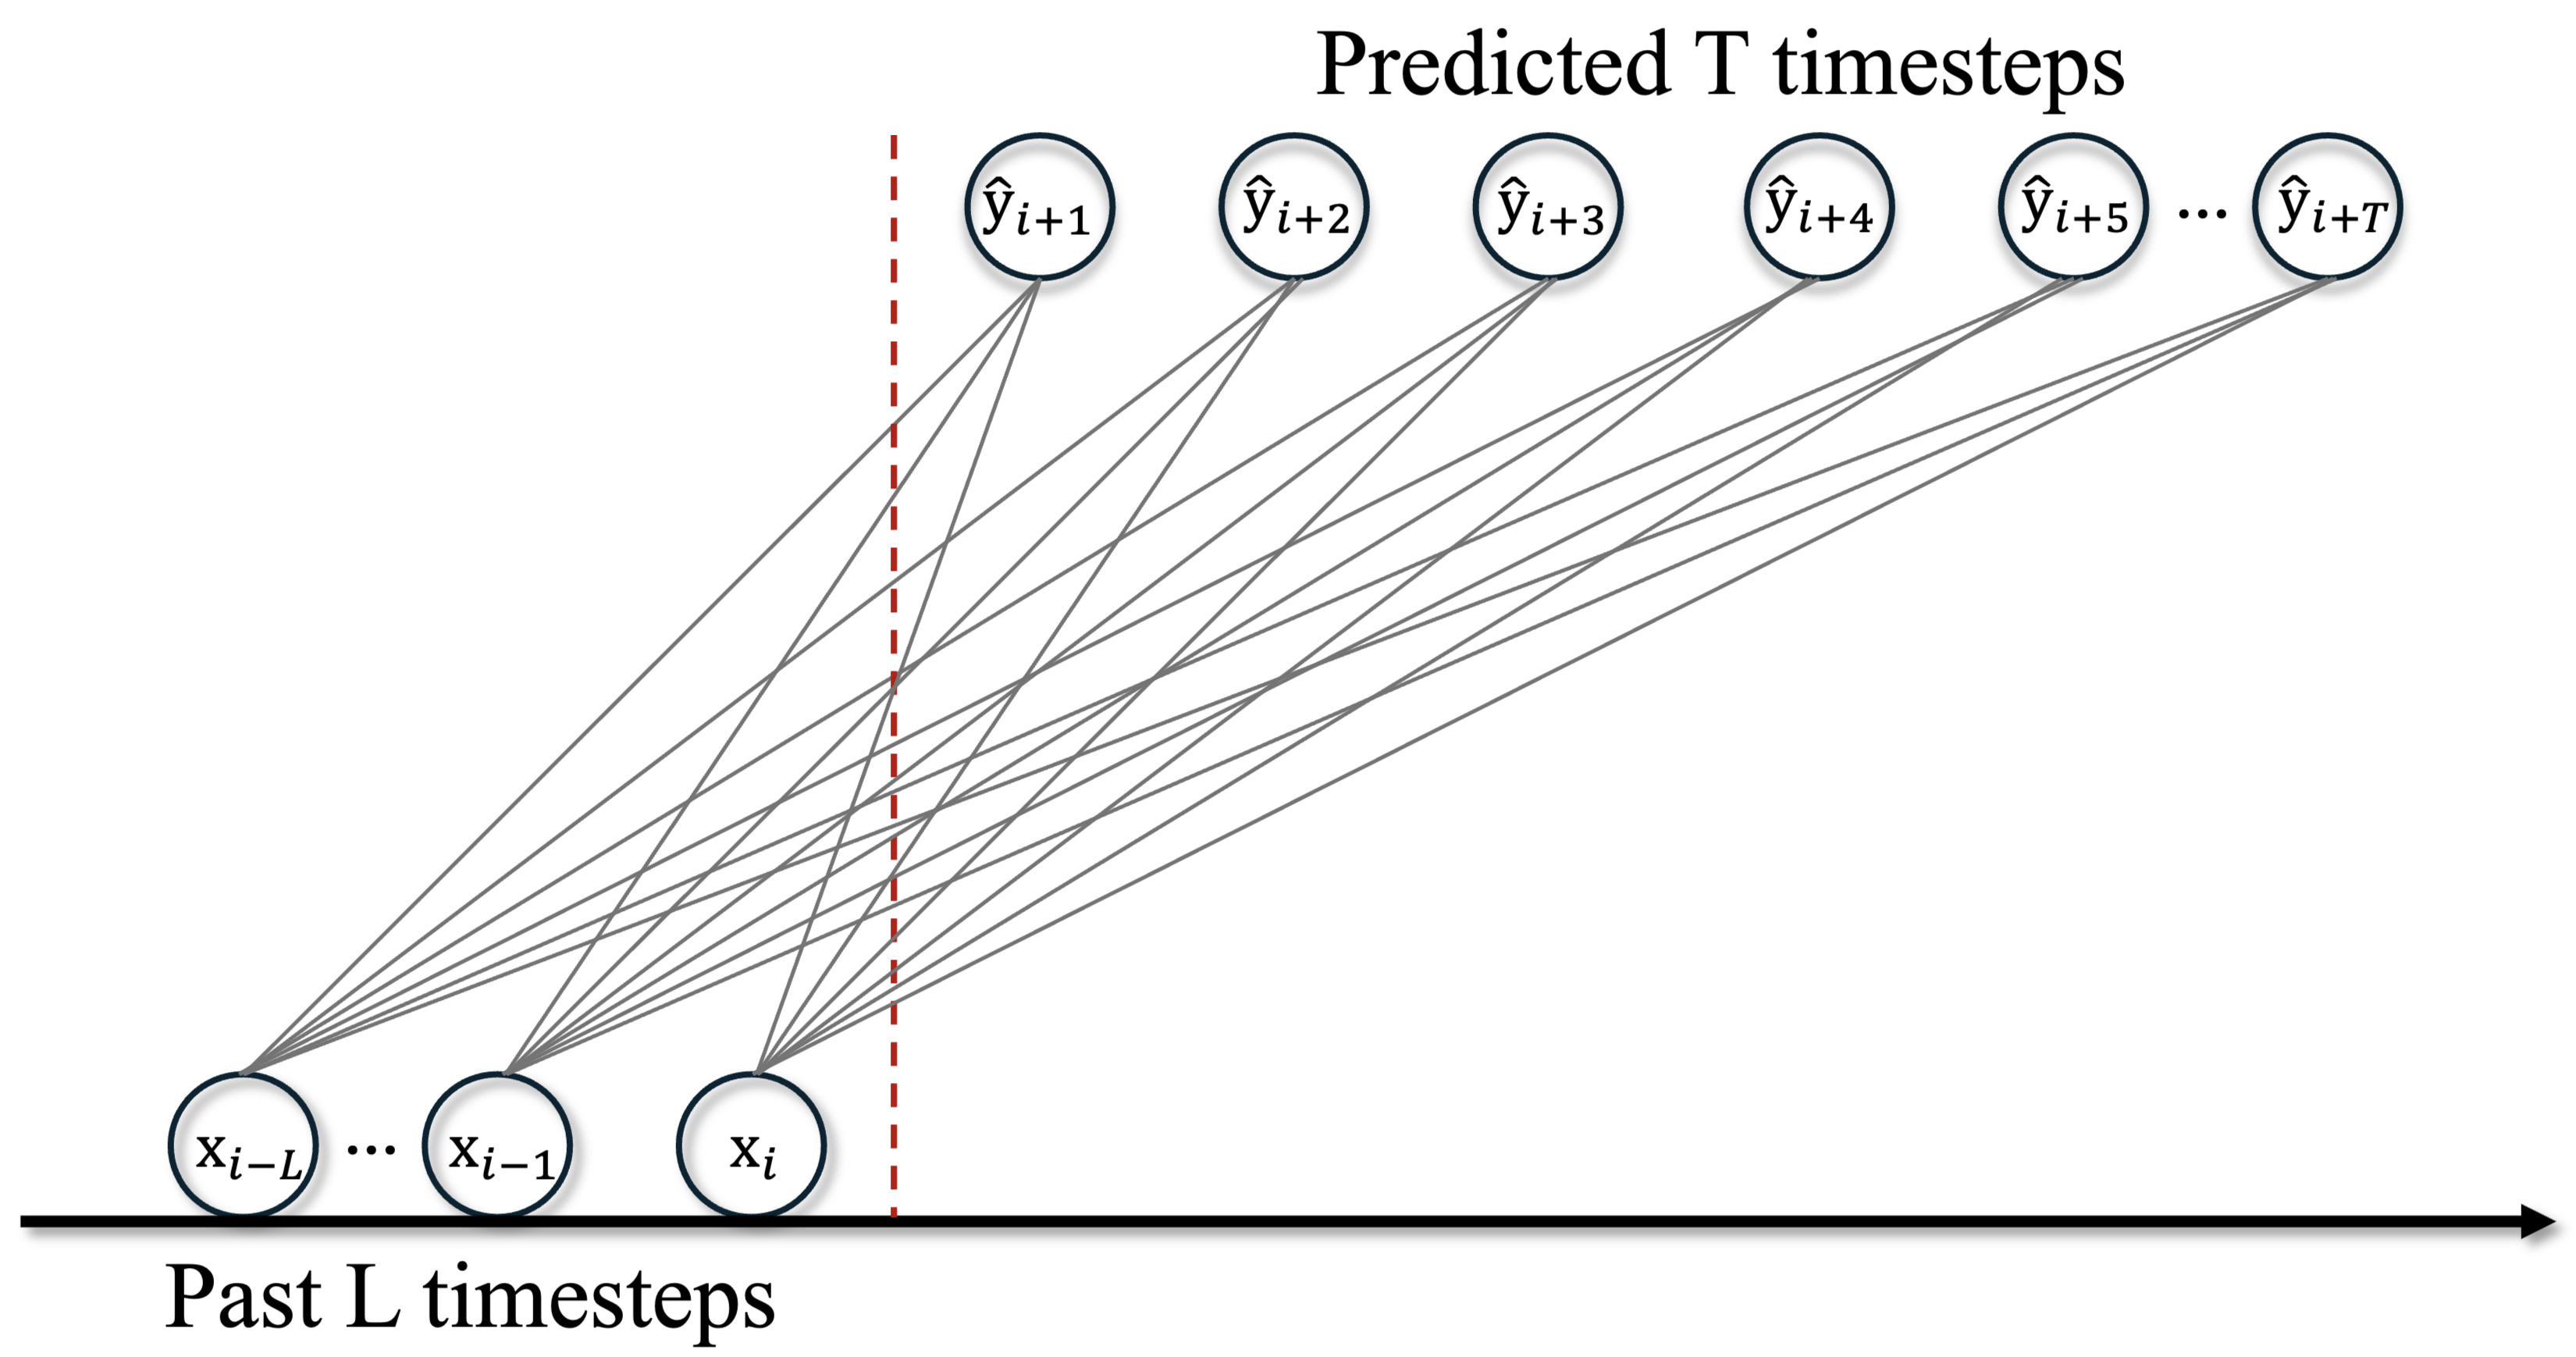
\includegraphics[width=85mm]{LTSF-Linear-illustration.png}
\caption{Illustration of LTSF-Linear models.}
\label{fig:linear}
\end{figure}

The Linear model employs a single-layer architecture that directly maps temporal dependencies through linear regression. DLinear enhances this by incorporating temporal decomposition, separating trend and seasonal components to handle long-term trajectories and cyclical patterns. NLinear further addresses non-stationarity through a normalization-linearization-denormalization process. These models serve as a strong baseline, proving that for many specific, smaller-scale datasets, simplicity and robustness often outweigh architectural complexity. However, they remain limited by their inability to transfer knowledge across different domains, relying solely on the patterns present in the specific formulation of the training data.

\subsection{TimeGPT: Bridging the gap with foundation models}

While traditional Transformers faced the limitations described in Section 3.1, TimeGPT \cite{GM2023} overcomes these hurdles through a fundamental paradigm shift: \textit{scale} and \textit{reprogramming}. Unlike standard Transformers trained from scratch on single datasets, TimeGPT is a foundation model pre-trained on over 100 billion data points across diverse domains (finance, weather, energy, etc.).

This massive pre-training allows TimeGPT to learn universal temporal patterns that generalize across different time series, effectively addressing the data-hunger and overfitting issues typical of standard Transformers. Furthermore, TimeGPT employs a specialized Transformer-based encoder-decoder architecture designed specifically for time series. It utilizes local positional encodings and a customized attention mechanism that are explicitly engineered to handle the sequential nature of time-series data, thereby mitigating the permutation-invariance problem found in generic NLP-based Transformers.

By combining the powerful representational learning of Transformers with specialized architectural inductive biases and massive scale, TimeGPT offers the best of both worlds: the generalization capability of large language models and the precision required for numerical forecasting. This allows for zero-shot inference that is both accurate and computationally efficient, contrasting sharply with the heavy training costs of traditional deep learning approaches.


\section{LLM based time series forecasting}
\subsection{Novel implementation on Gamcheon dataset}

In this study, we present a comprehensive and pioneering analysis of water level forecasting for the Gamcheon dataset. Our research uniquely integrates classical time series models, linear models, and large language model (LLM)-based approaches to create a robust forecasting framework. As shown in Table \ref{tab:data}, we utilize multiple environmental variables from two key monitoring stations - Seounju-kyo and Gumi-si. 

\begin{table}[H]
\centering
\begin{tabular}{|c|c|c|}
\hline
\textbf{Data} & \textbf{Gauging Station} & \textbf{Application} \\
\hline
Precipitation &  Seounju-kyo & Input \\
Water level &  Seounju-kyo & Input \\
\hline
Water level & Seounju-kyo & Output \\
\hline
\end{tabular}
\caption{Input data and output data for Seounju-kyo checkpoint.}
\label{tab:data}
\end{table}

The input features primarily include precipitation data and water level measurements from the Seounju-kyo station. Initial exploratory analysis considered auxiliary meteorological variables (Wind, Temperature, Humidity) from the Gumi-si station; however, feature importance analysis revealed that rainfall metrics were the dominant predictors for water level fluctuations in this catchment. Consequently, to maintain model parsimony and focus on the most causal factors, the final experimental setup relies exclusively on historical water levels and engineered rainfall features. Only Seounju-kyo station data serves as both input and target variables.

\subsection{Scenario-based comparative analysis}

We adopt a scenario-based comparative analysis approach to thoroughly explore different forecasting paradigms applied to the Gamcheon dataset, showcasing the evolution from classical models to advanced LLM-based methodologies. This analysis highlights the value of each model type in addressing the complexities of water level forecasting. The novelty of this work lies in the integration of traditional, simplified, and advanced techniques to comprehensively tackle the challenges of environmental time series forecasting. The diverse methodologies, tailored experimental scenarios, and the unique dataset context combine to make this study a significant contribution to the field of time series analysis.

\subsection{Experiment setup}

\paragraph{Data Periods and Scenarios}
To ensure a rigorous comparative analysis, we define three scenarios targeting different evaluation regimes. \textbf{Scenario 1} (Classical models: SARIMAX~\cite{BJ2015}, Prophet~\cite{TL2018}) and \textbf{Scenario 2} (LTSF-Linear models: Linear, DLinear, NLinear~\cite{ZCLX23}) focus on the intensive flood event of \textbf{July 25 to September 10, 2024 (KST)}. This period was selected to evaluate model performance during critical monsoon activity. Linear models are trained for 10 epochs using MSE loss. \textbf{Scenario 3} evaluates TimeGPT in a zero-shot setting over the full hydrological cycle from \textbf{August 2023 to July 2024}, testing robustness across diverse seasonal conditions. For the enhanced \textit{TimeGPT (ex)}, we incorporate 36-hour cumulative rainfall and 6-hour rainfall intensity. These features were selected via correlation analysis to effectively capture soil saturation lags and flash flood dynamics, respectively.

\paragraph{Evaluation Protocol}
We employ a \emph{pure rolling-origin} evaluation protocol. For each forecast origin $t$, models use the last $L$ days of observations to produce an $H$-day forecast. We test three horizon configurations $(L, H)$: short-term $[7, 3]$, medium-term $[30, 7]$, and long-term $[180, 30]$. For TimeGPT, no gradient updates are performed, validating its capability as a general-purpose foundation model without overfitting to the specific historical record.

\subsection{Evaluation metrics}

To quantitatively evaluate model performance, three commonly used metrics are employed: Mean Absolute Error (MAE), Nash–Sutcliffe Efficiency (NSE), and Root Mean Square Error (RMSE). Their mathematical formulations are as follows:

\begin{equation}
\text{MAE} = \frac{1}{n} \sum_{i=1}^{n} \left| y_i - \hat{y}_i \right|
\label{eq:mae}
\end{equation}

\begin{equation}
\text{NSE} = 1 - \frac{\sum_{i=1}^{n} (y_i - \hat{y}_i)^2}{\sum_{i=1}^{n} (y_i - \bar{y})^2}
\label{eq:nse}
\end{equation}

\begin{equation}
\text{RMSE} = \sqrt{\frac{1}{n} \sum_{i=1}^{n} (y_i - \hat{y}_i)^2}
\label{eq:rmse}
\end{equation}

where $y_i$ denotes the observed water level, $\hat{y}_i$ the predicted water level, $\bar{y}$ the mean of observed values, and $n$ the total number of samples.

MAE measures the average magnitude of prediction errors regardless of their direction; a smaller MAE indicates higher predictive accuracy.  
NSE evaluates how well the predicted time series matches the observed data, with values closer to 1 representing better model performance.  
RMSE penalizes larger errors more heavily and thus is sensitive to outliers; a lower RMSE indicates improved overall prediction consistency.

\section{Results and analyses}

In this section, we present the results of the experiments conducted in Scenarios 1--3. The results are summarized in table \ref{tab:Model Performance Metrics} and figures, with detailed explanations provided.

\begin{table}[H]
\centering
\captionsetup{labelsep=period}
\caption{Performance metrics for Scenarios 1, 2, and 3 at the Seounju-kyo checkpoint.}
\label{tab:model_performance}
\footnotesize
\begin{tabular}{!{\color{black}\vrule}l!{\color{black}\vrule}l!{\color{black}\vrule}c!{\color{black}\vrule}c!{\color{black}\vrule}c!{\color{black}\vrule}}
\arrayrulecolor{black}\specialrule{.1em}{.1em}{.1em}
\rowcolor{gray!40} \textbf{Stage} & \textbf{Metric} & \textbf{[7, 3] days} & \textbf{[30, 7] days} & \textbf{[180, 30] days} \\
\arrayrulecolor{black}\specialrule{.1em}{.1em}{.1em}
\multicolumn{5}{!{\color{black}\vrule}c!{\color{black}\vrule}}{\cellcolor{gray!20}\textbf{Scenario 1}} \\
\arrayrulecolor{gray}\specialrule{.1em}{.1em}{.1em}
\multirow{3}{*}{SARIMAX} 
& MAE  & 0.0370 & 0.0389  & 0.0668 \\
& NSE  & -0.2113 & -0.2432 & -2.7908 \\
& RMSE & 0.0547 & 0.0450 & 0.0726 \\

\arrayrulecolor{gray}\specialrule{.1em}{.1em}{.1em}
\multirow{3}{*}{Prophet} 
& MAE  & 0.0541  & 0.1433  & 0.2628  \\
& NSE  & -1.5487  & -15.3025  & -49.9023  \\
& RMSE & 0.0794  & 0.1630  & 0.2659  \\

\arrayrulecolor{black}\specialrule{.1em}{.1em}{.1em}
\multicolumn{5}{!{\color{black}\vrule}c!{\color{black}\vrule}}{\cellcolor{gray!20}\textbf{Scenario 2}} \\
\arrayrulecolor{gray}\specialrule{.1em}{.1em}{.1em}

\multirow{3}{*}{Linear}  
& MAE  & 0.0579 & 0.1157  & 0.3489  \\
& NSE  & 0.3496 & -0.3836 & -5.2617 \\
& RMSE & 0.1245 & 0.1815  & 0.3862  \\
\arrayrulecolor{gray}\specialrule{.1em}{.1em}{.1em}

\multirow{3}{*}{DLinear} 
& MAE  & 0.0695 & 0.1493  & 0.1026  \\
& NSE  & 0.2652 & -0.5586 & -0.4340 \\
& RMSE & 0.1323 & 0.1927  & 0.1848  \\
\arrayrulecolor{gray}\specialrule{.1em}{.1em}{.1em}

\multirow{3}{*}{NLinear} 
& MAE  & 0.0491 & 0.0677 & 0.1025  \\
& NSE  & 0.4070 & \textbf{0.1047}  & \underline{-0.1671} \\
& RMSE & 0.1188 & 0.1460  & 0.1667  \\
\arrayrulecolor{black}\specialrule{.1em}{.1em}{.1em}

\multicolumn{5}{!{\color{black}\vrule}c!{\color{black}\vrule}}{\cellcolor{gray!20}\textbf{Scenario 3}} \\
\arrayrulecolor{gray}\specialrule{.1em}{.1em}{.1em}
\multirow{3}{*}{TimeGPT} 
& MAE  & \textbf{0.0182} & \textbf{0.0233} & \textbf{0.0310} \\
& NSE  & \underline{0.5101} & \underline{0.0850} & \textbf{-0.0440} \\
& RMSE & \underline{0.0253} & \textbf{0.0346} & \textbf{0.0370} \\
\arrayrulecolor{gray}\specialrule{.1em}{.1em}{.1em}

\multirow{3}{*}{TimeGPT (ex)} 
& MAE  & \underline{0.0184} & \underline{0.0565} & \underline{0.0476} \\
& NSE  & \textbf{0.5598} & -7.2155 & -1.5723 \\
& RMSE & \textbf{0.0240} & \underline{0.1038} & \underline{0.0581} \\
\arrayrulecolor{black}\specialrule{.1em}{.1em}{.1em}
\end{tabular}
\label{tab:Model Performance Metrics}
\end{table}

We evaluate the performance of the models using key metrics, including NSE, RMSE, and MAE, across different prediction window and forecast horizon combinations of [7, 3] days, [30, 7] days, and [180, 30] days. Scenario 1 evaluates classical statistical models, Scenario 2 compares the Linear, DLinear, and NLinear models, and Scenario 3 utilizes the Time-LLM approach. Bold values indicate the best performance and underlined values indicate the second-best performance for each metric.

\subsection{Results and analyses on Scenario 1}

In Scenario~1, the SARIMAX and Prophet models were evaluated as classical statistical baselines for water level forecasting. The SARIMAX model, shown in Figure~\ref{fig:SARIMAX_predictions}, produces smooth and stable forecasts with limited fluctuation, reflecting its tendency to revert toward the mean when exogenous variables (e.g., precipitation) vary only slightly. While this conservatism yields stable short-term estimates, it limits responsiveness to abrupt hydrological changes.

The Prophet model (Figure~\ref{fig:prophet_model_predictions}) captures seasonal and trend components more dynamically, resulting in higher short-term sensitivity but frequent overestimation for longer horizons. In each plot, the black line represents observed water levels and the dashed lines denote model predictions for varying window sizes. Despite its flexibility, Prophet often fails to capture sudden water-level surges caused by intense rainfall events. Both models incorporated precipitation and its squared term as external regressors to reflect non-linear rainfall effects, which improved robustness but not sufficiently for extreme conditions.

\begin{figure}[H]
    \centering
    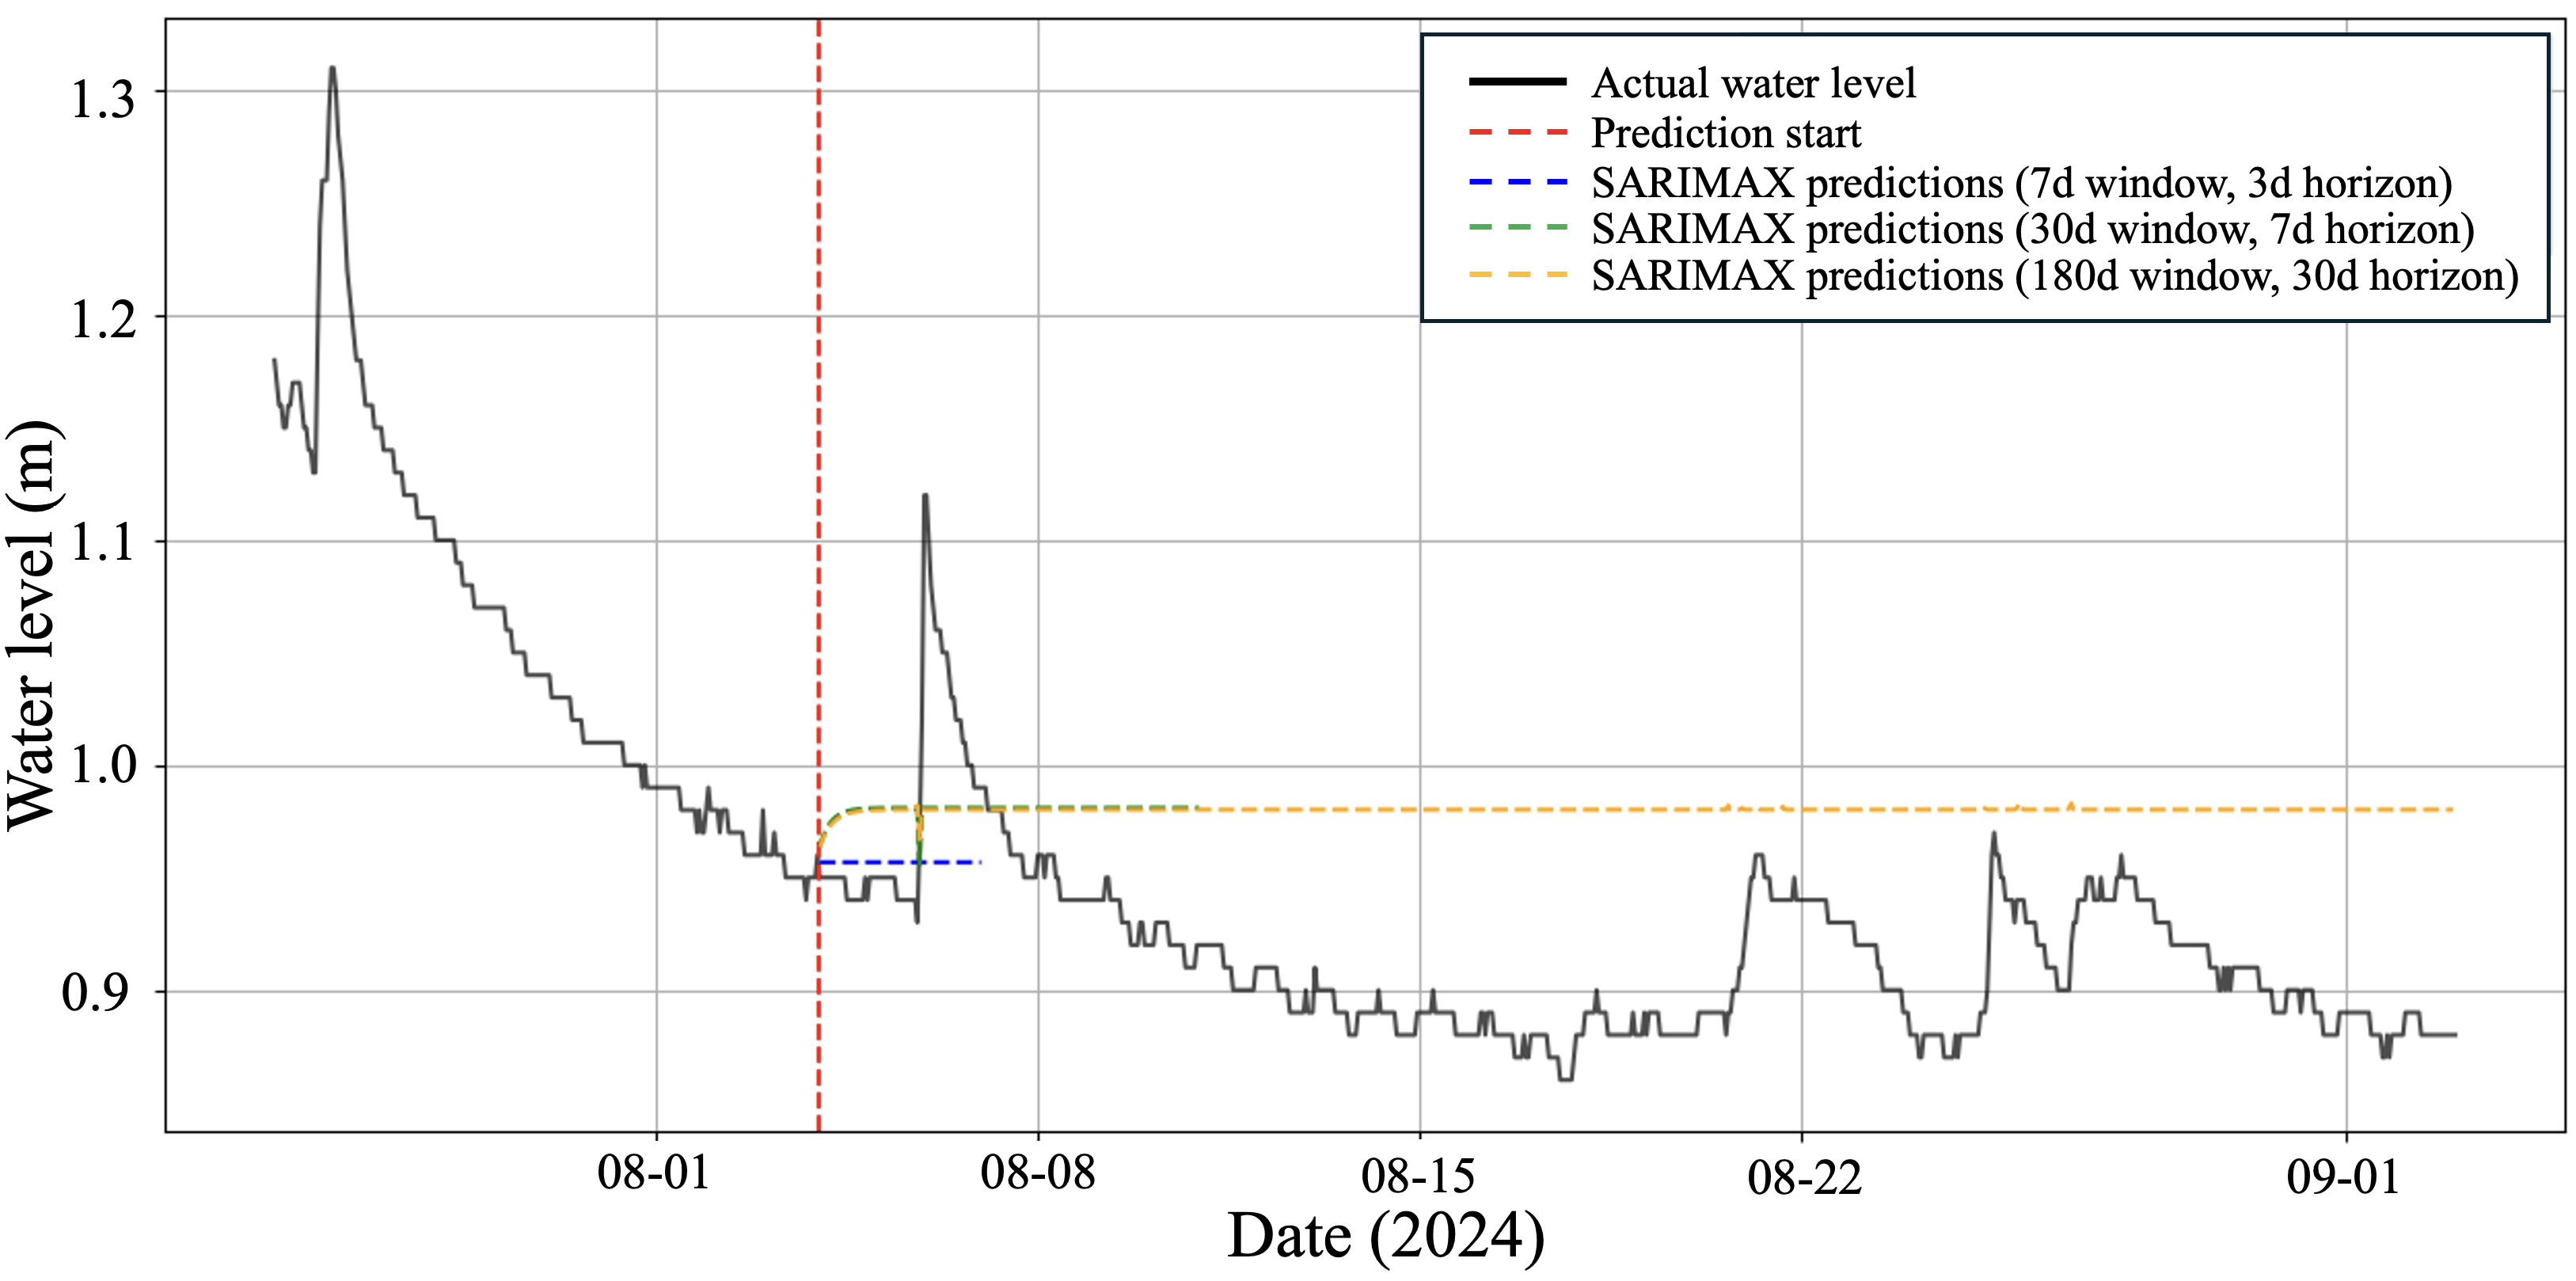
\includegraphics[width=85mm]{SARIMAX_predictions.png}
    \caption{Water level predictions using the SARIMAX model.}
    \label{fig:SARIMAX_predictions}
\end{figure}

\begin{figure}[H]
    \centering
    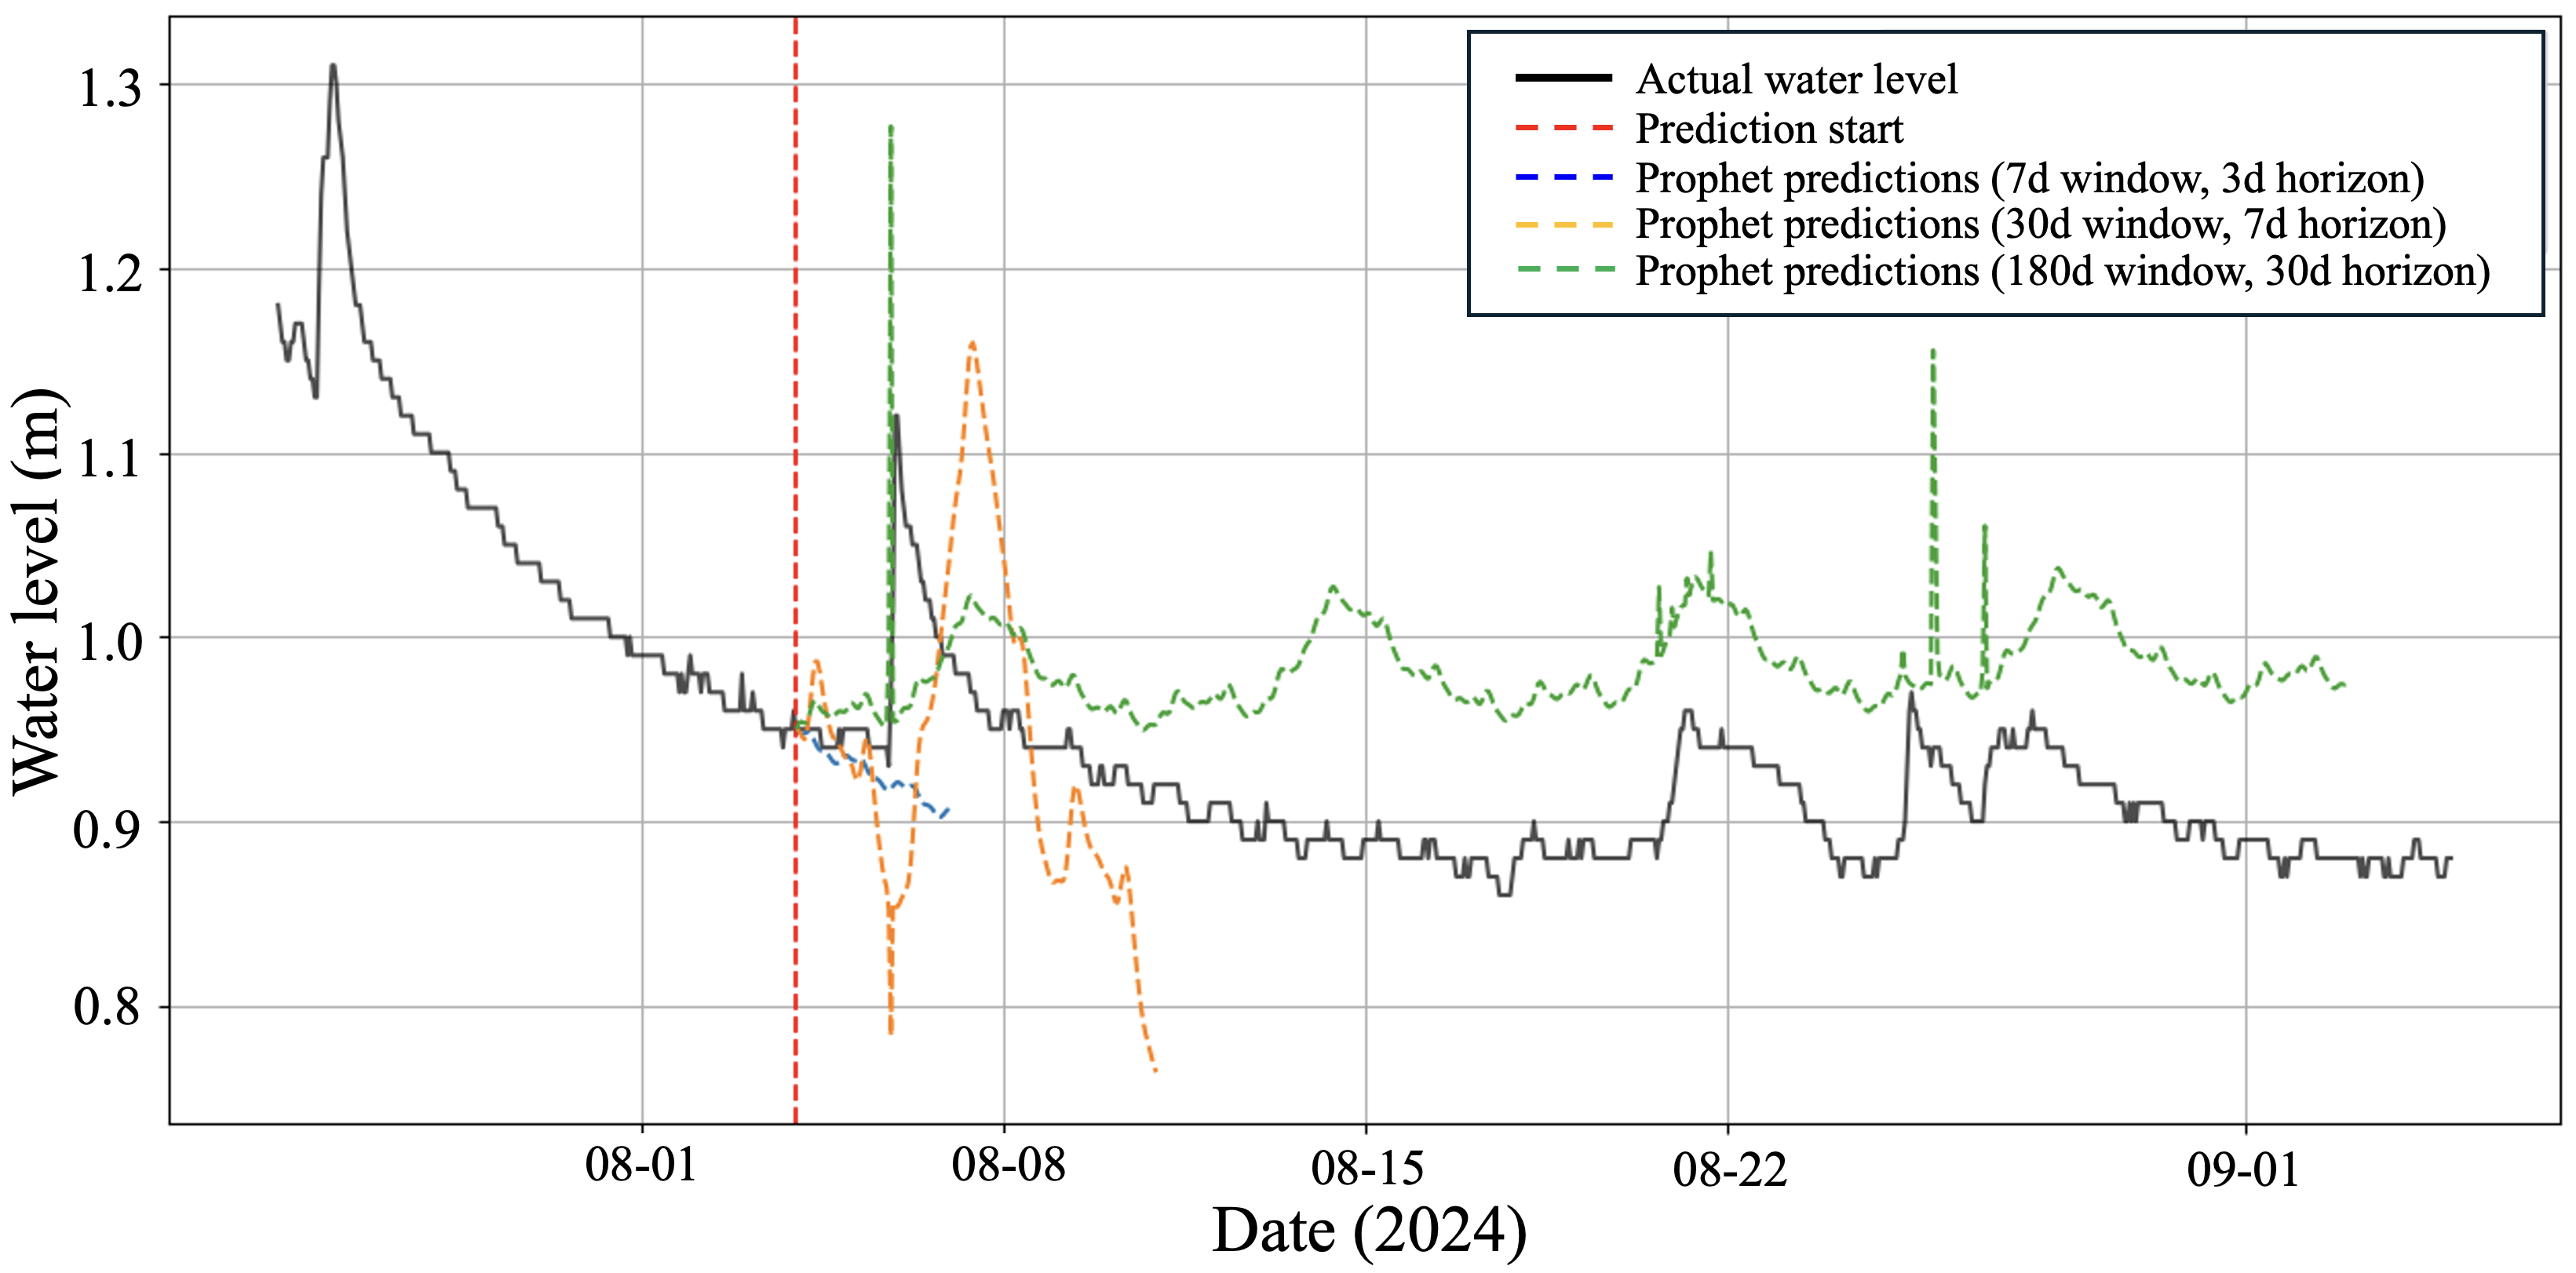
\includegraphics[width=85mm]{Prophet_predictions.png}
    \caption{Water level predictions using the Prophet model.}
    \label{fig:prophet_model_predictions}
\end{figure}

\subsection{Results and analyses on Scenario 2}
Scenario~2 compares three linear architectures—Linear, DLinear, and NLinear—to evaluate their efficiency in capturing temporal dependencies. The Linear model (Figure~\ref{fig:linear_model_predictions}) serves as a baseline, applying a direct linear transformation between past and future values. It performs reasonably well for short-term forecasts but degrades rapidly as the prediction horizon extends.

The DLinear model (Figure~\ref{fig:dlinear_model_predictions}) improves upon this by decomposing inputs into trend and seasonal components, yielding lower RMSE values for medium- and long-term forecasts. This decomposition enables the model to capture persistent seasonal cycles while maintaining computational simplicity.

Among the three, the NLinear model (Figure~\ref{fig:nlinear_model_predictions}) achieves the best overall performance, particularly for short-term forecasts. By normalizing each sequence with respect to the last observed value, it effectively captures relative variations and mitigates distributional shifts, resulting in higher NSE and lower MAE scores. This stability across varying horizons demonstrates the robustness of normalization-based approaches for non-stationary environmental data.

\begin{figure}[H]
    \centering
    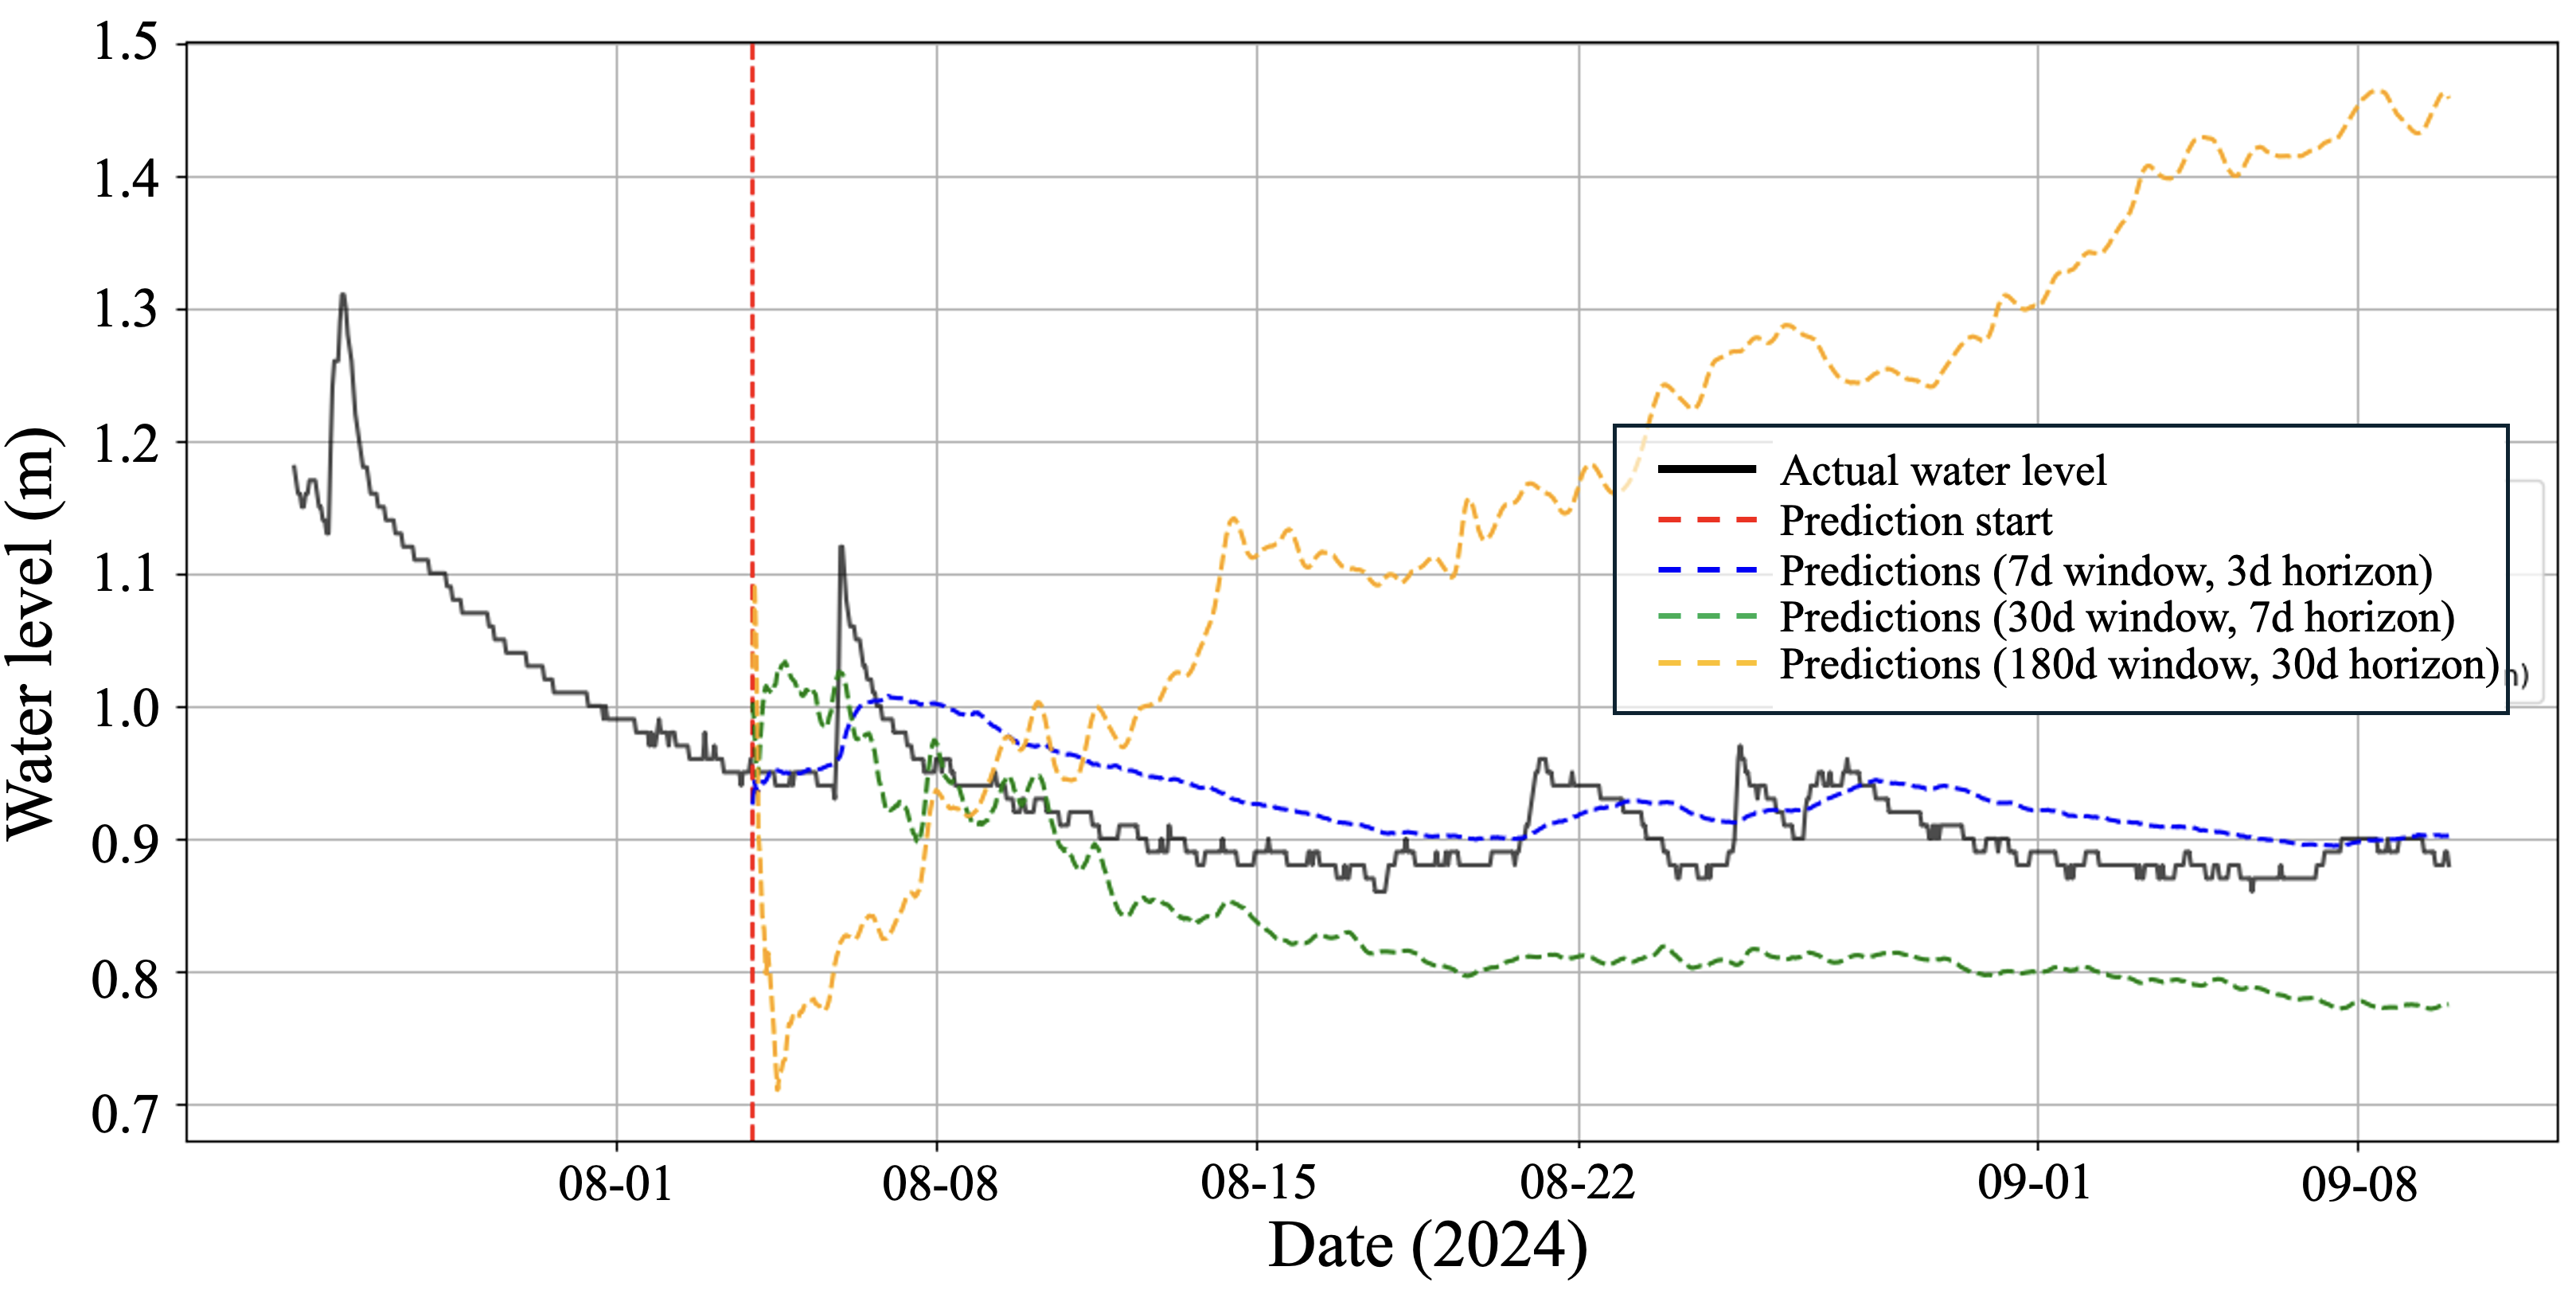
\includegraphics[width=85mm]{Linear_predictions.png}
    \caption{Water level predictions using the Linear model.}
    \label{fig:linear_model_predictions}
\end{figure}

\begin{figure}[H]
    \centering
    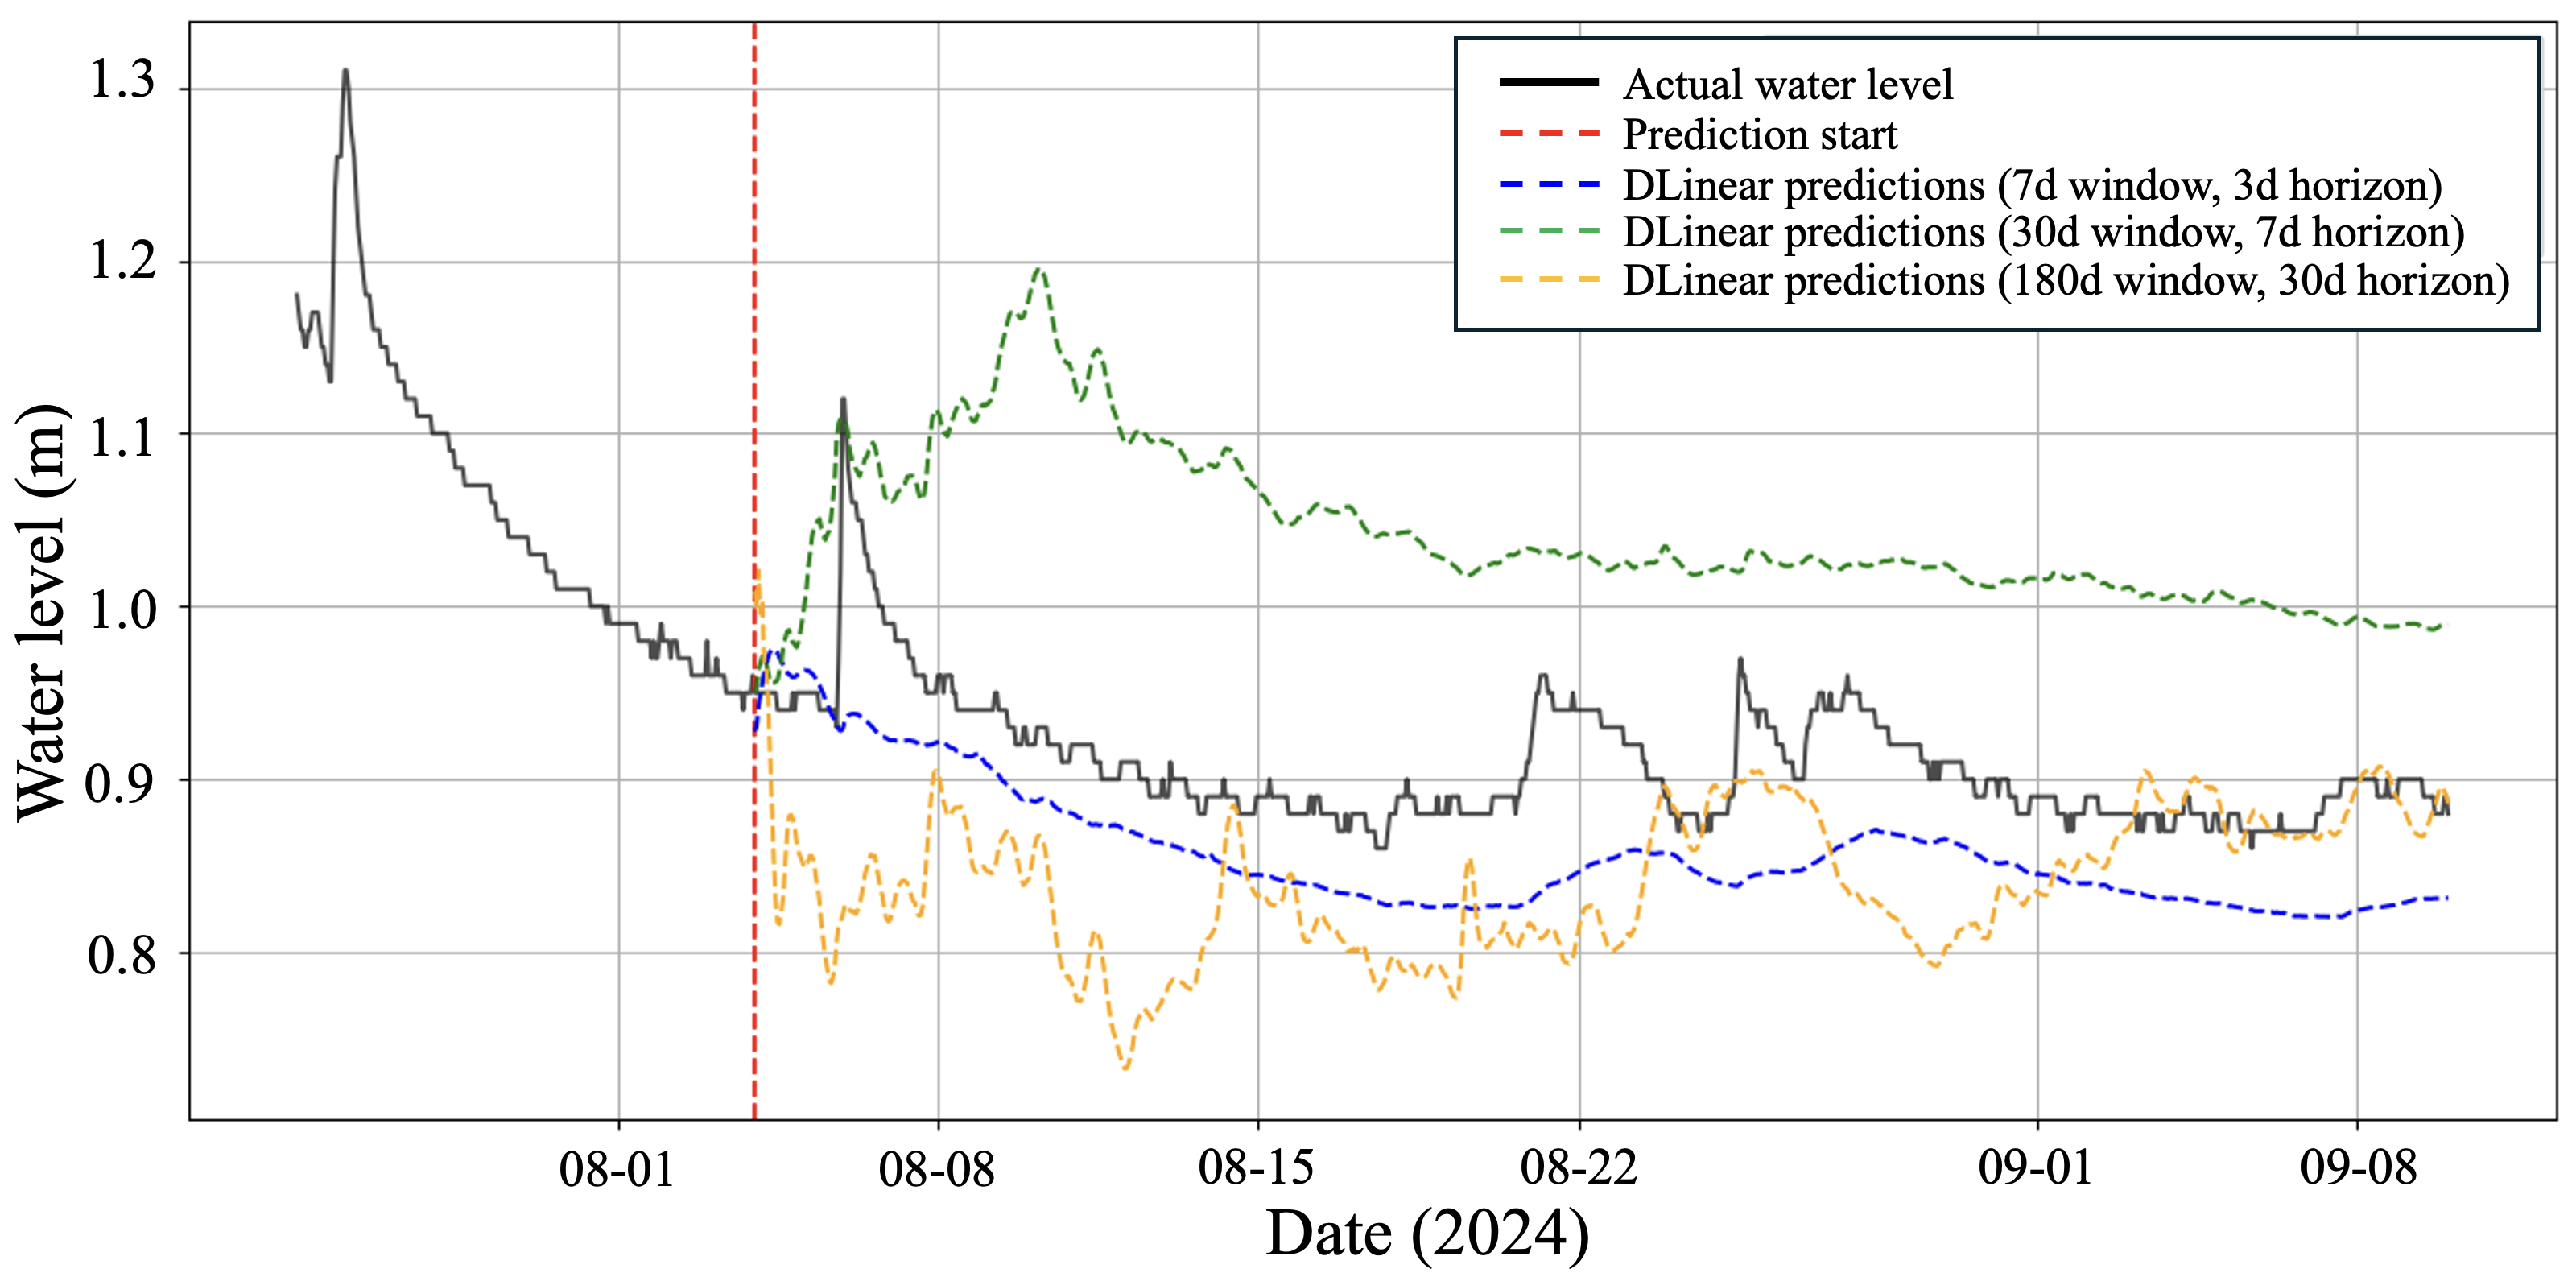
\includegraphics[width=85mm]{DLinear_predictions.png}
    \caption{Water level predictions using the DLinear model.}
    \label{fig:dlinear_model_predictions}
\end{figure}

\begin{figure}[H]
    \centering
    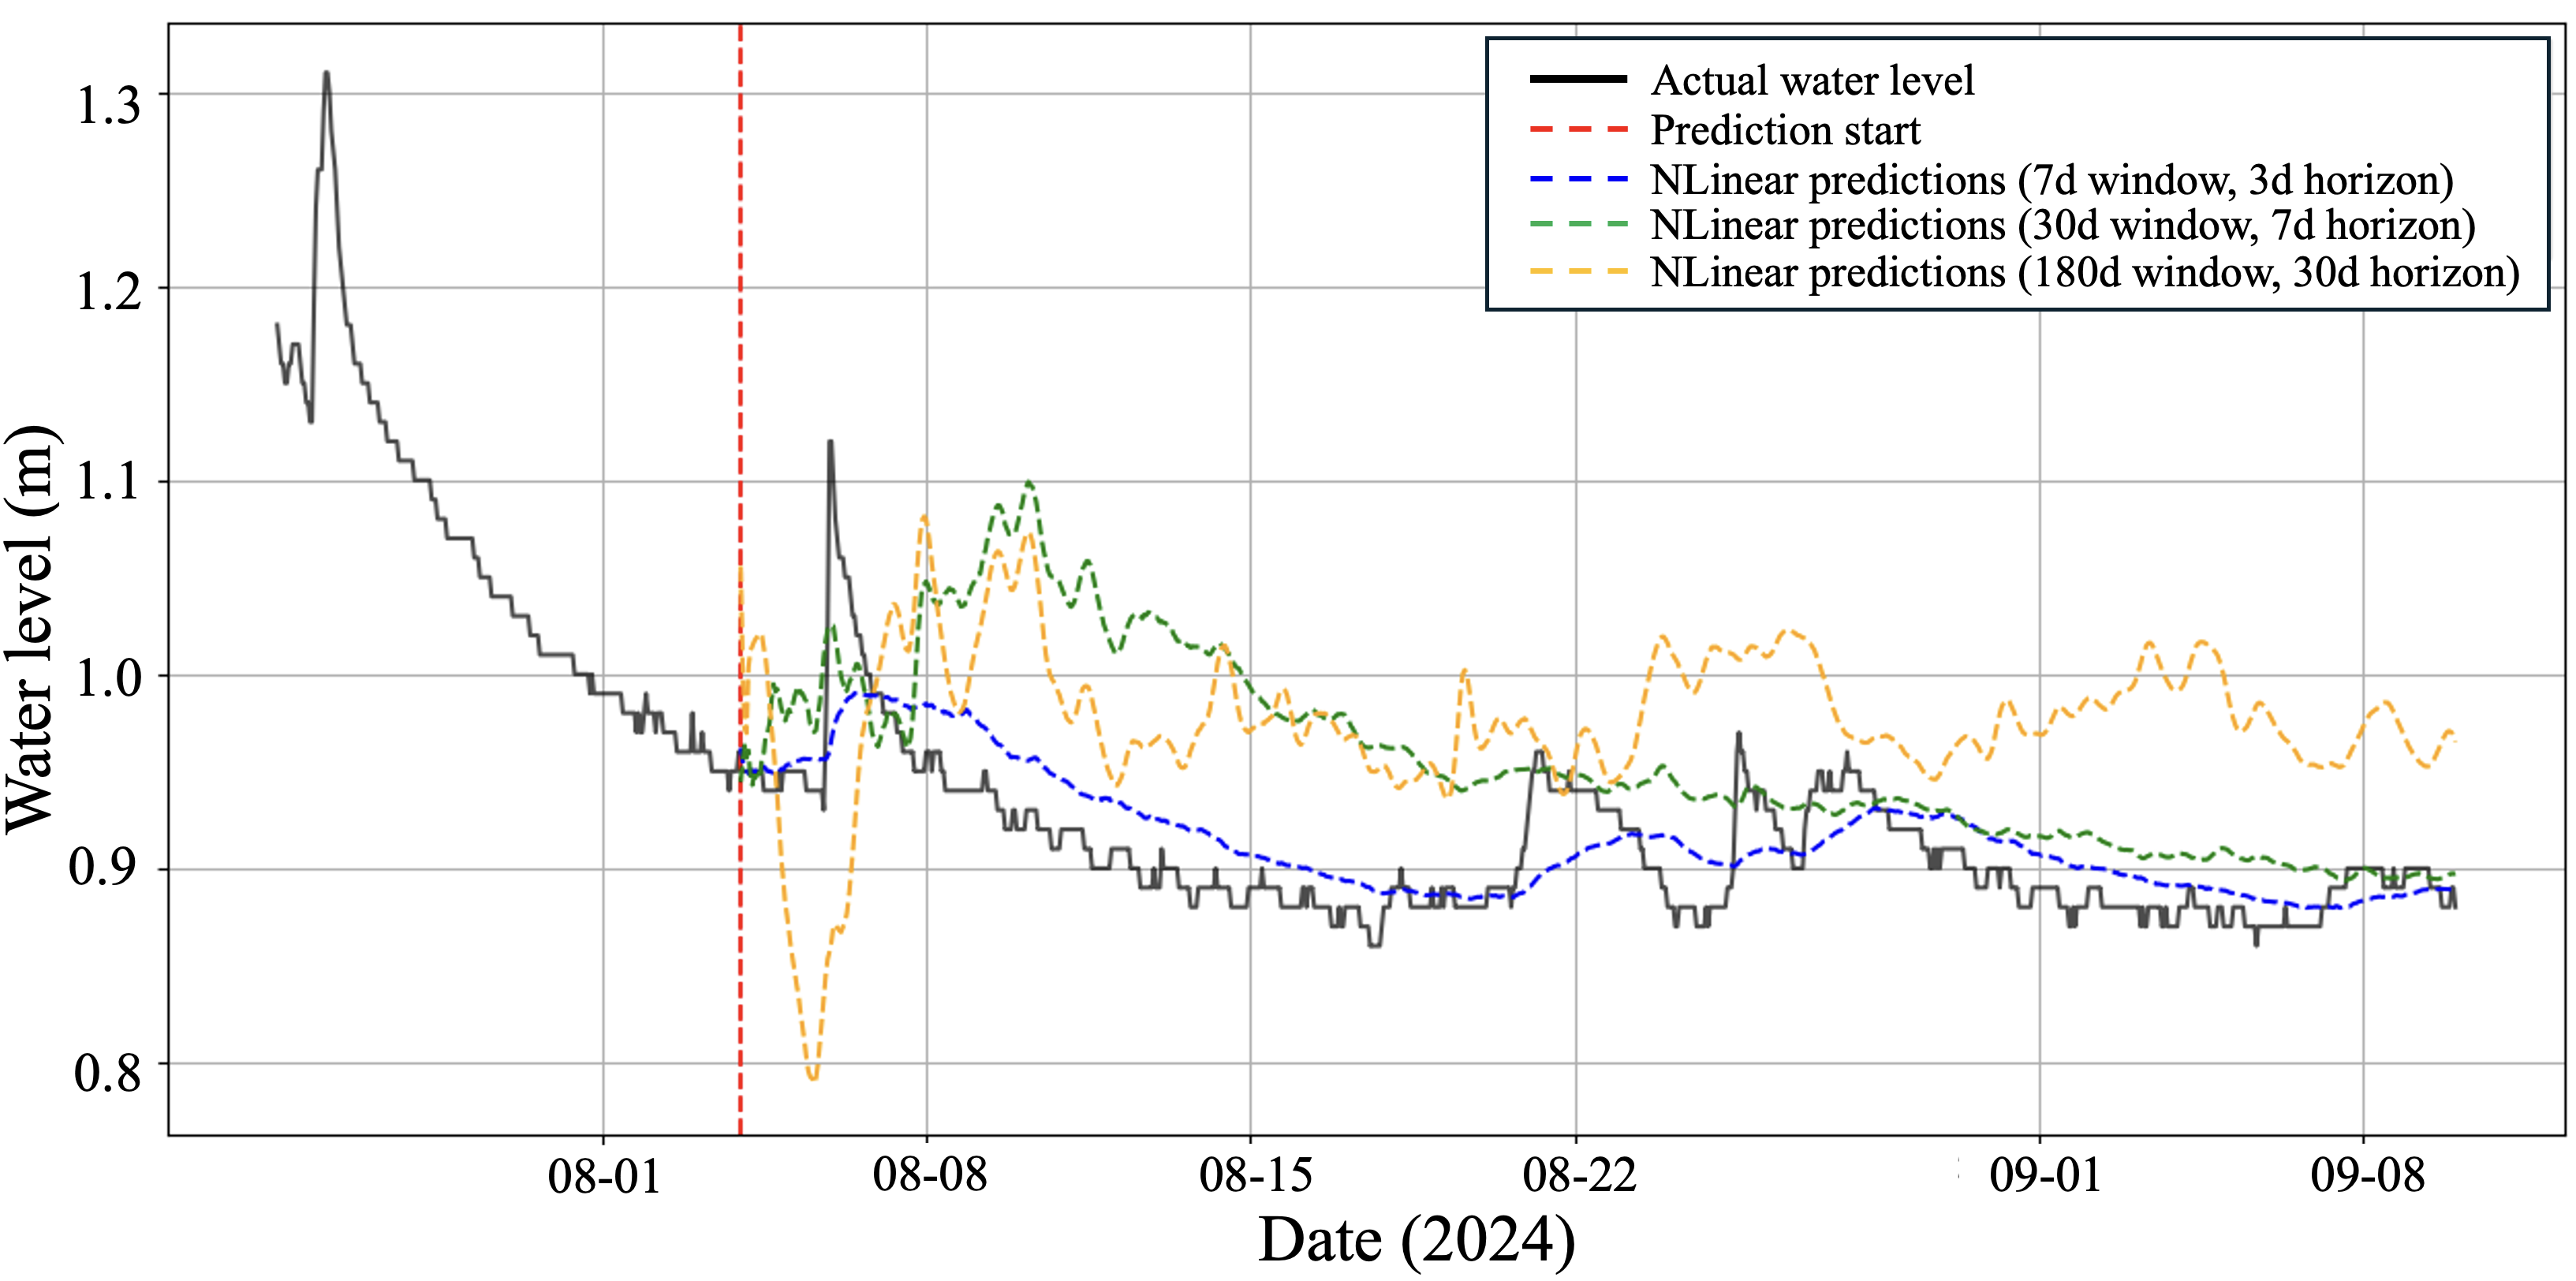
\includegraphics[width=85mm]{NLinear_predictions.png}
    \caption{Water level predictions using the NLinear model.}
    \label{fig:nlinear_model_predictions}
\end{figure}


\subsection{Results and analyses on Scenario 3}

Scenario~3 evaluates the performance of the pre-trained Time GPT model and its enhanced version with external rainfall variables, TimeGPT (ex). Both models demonstrate substantial improvements over the classical and linear approaches discussed earlier.

The base TimeGPT model exhibits strong predictive capability across different temporal horizons. As shown in Figure~\ref{fig:time_gpt_predictions}, it achieves an NSE of 0.5101 for the short-term window [7,3] with remarkably low RMSE (0.0253) and MAE (0.0182), indicating precise short-term forecasting. Performance remains stable for medium-term [30,7] predictions (NSE~0.0850; RMSE~0.0346), and—unlike statistical models—TimeGPT retains accuracy even in long-term forecasts [180,30] with NSE~–0.0440. These results highlight the model’s strength in learning complex temporal dependencies while maintaining computational efficiency.

The extended model, TimeGPT~(ex), integrates precipitation variables (36-hour cumulative and 6-hour intensity) to capture hydrometeorological influences. Figure~\ref{fig:time_gpt_predictions_ex} shows that this integration enhances short-term accuracy, achieving the highest NSE (0.5598) and lowest RMSE (0.0240) among all tested models. While TimeGPT~(ex) exhibits slightly higher sensitivity and wider confidence intervals for longer horizons, this responsiveness enables improved detection of extreme rainfall-driven fluctuations that the base model often smooths out.

\begin{figure}[H]
    \centering
    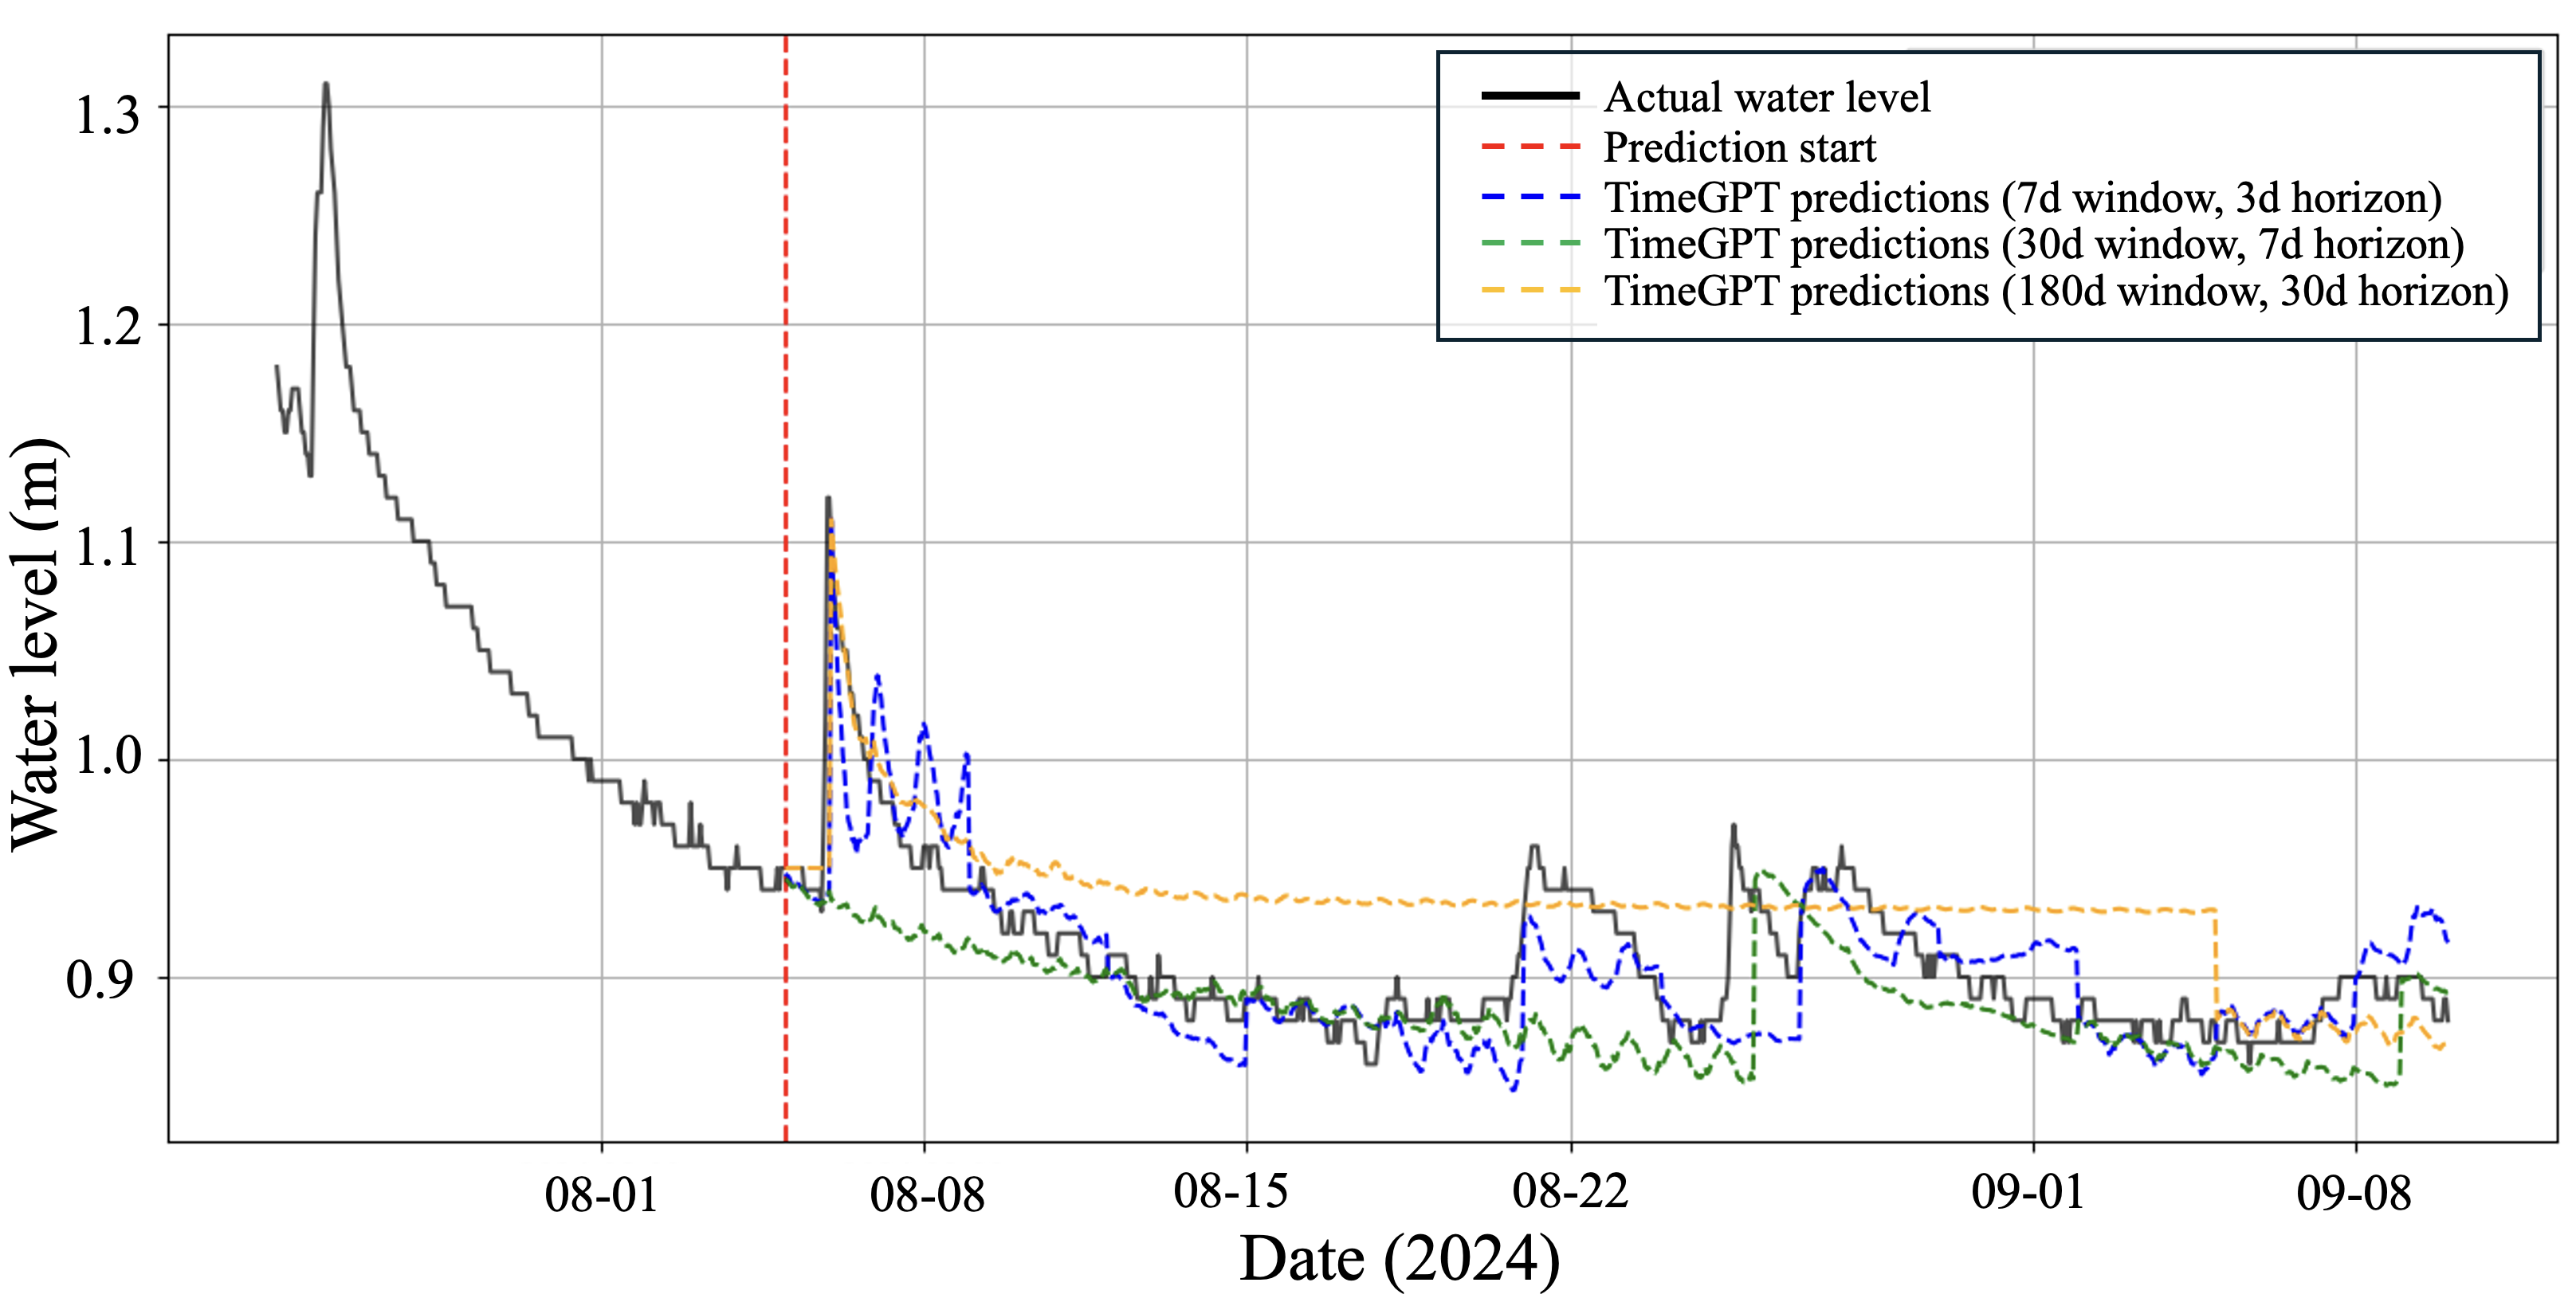
\includegraphics[width=85mm]{TimeGPT_predictions.png}
    \caption{Water level predictions using the TimeGPT model.}
    \label{fig:time_gpt_predictions}
\end{figure}

\begin{figure}[H]
    \centering
    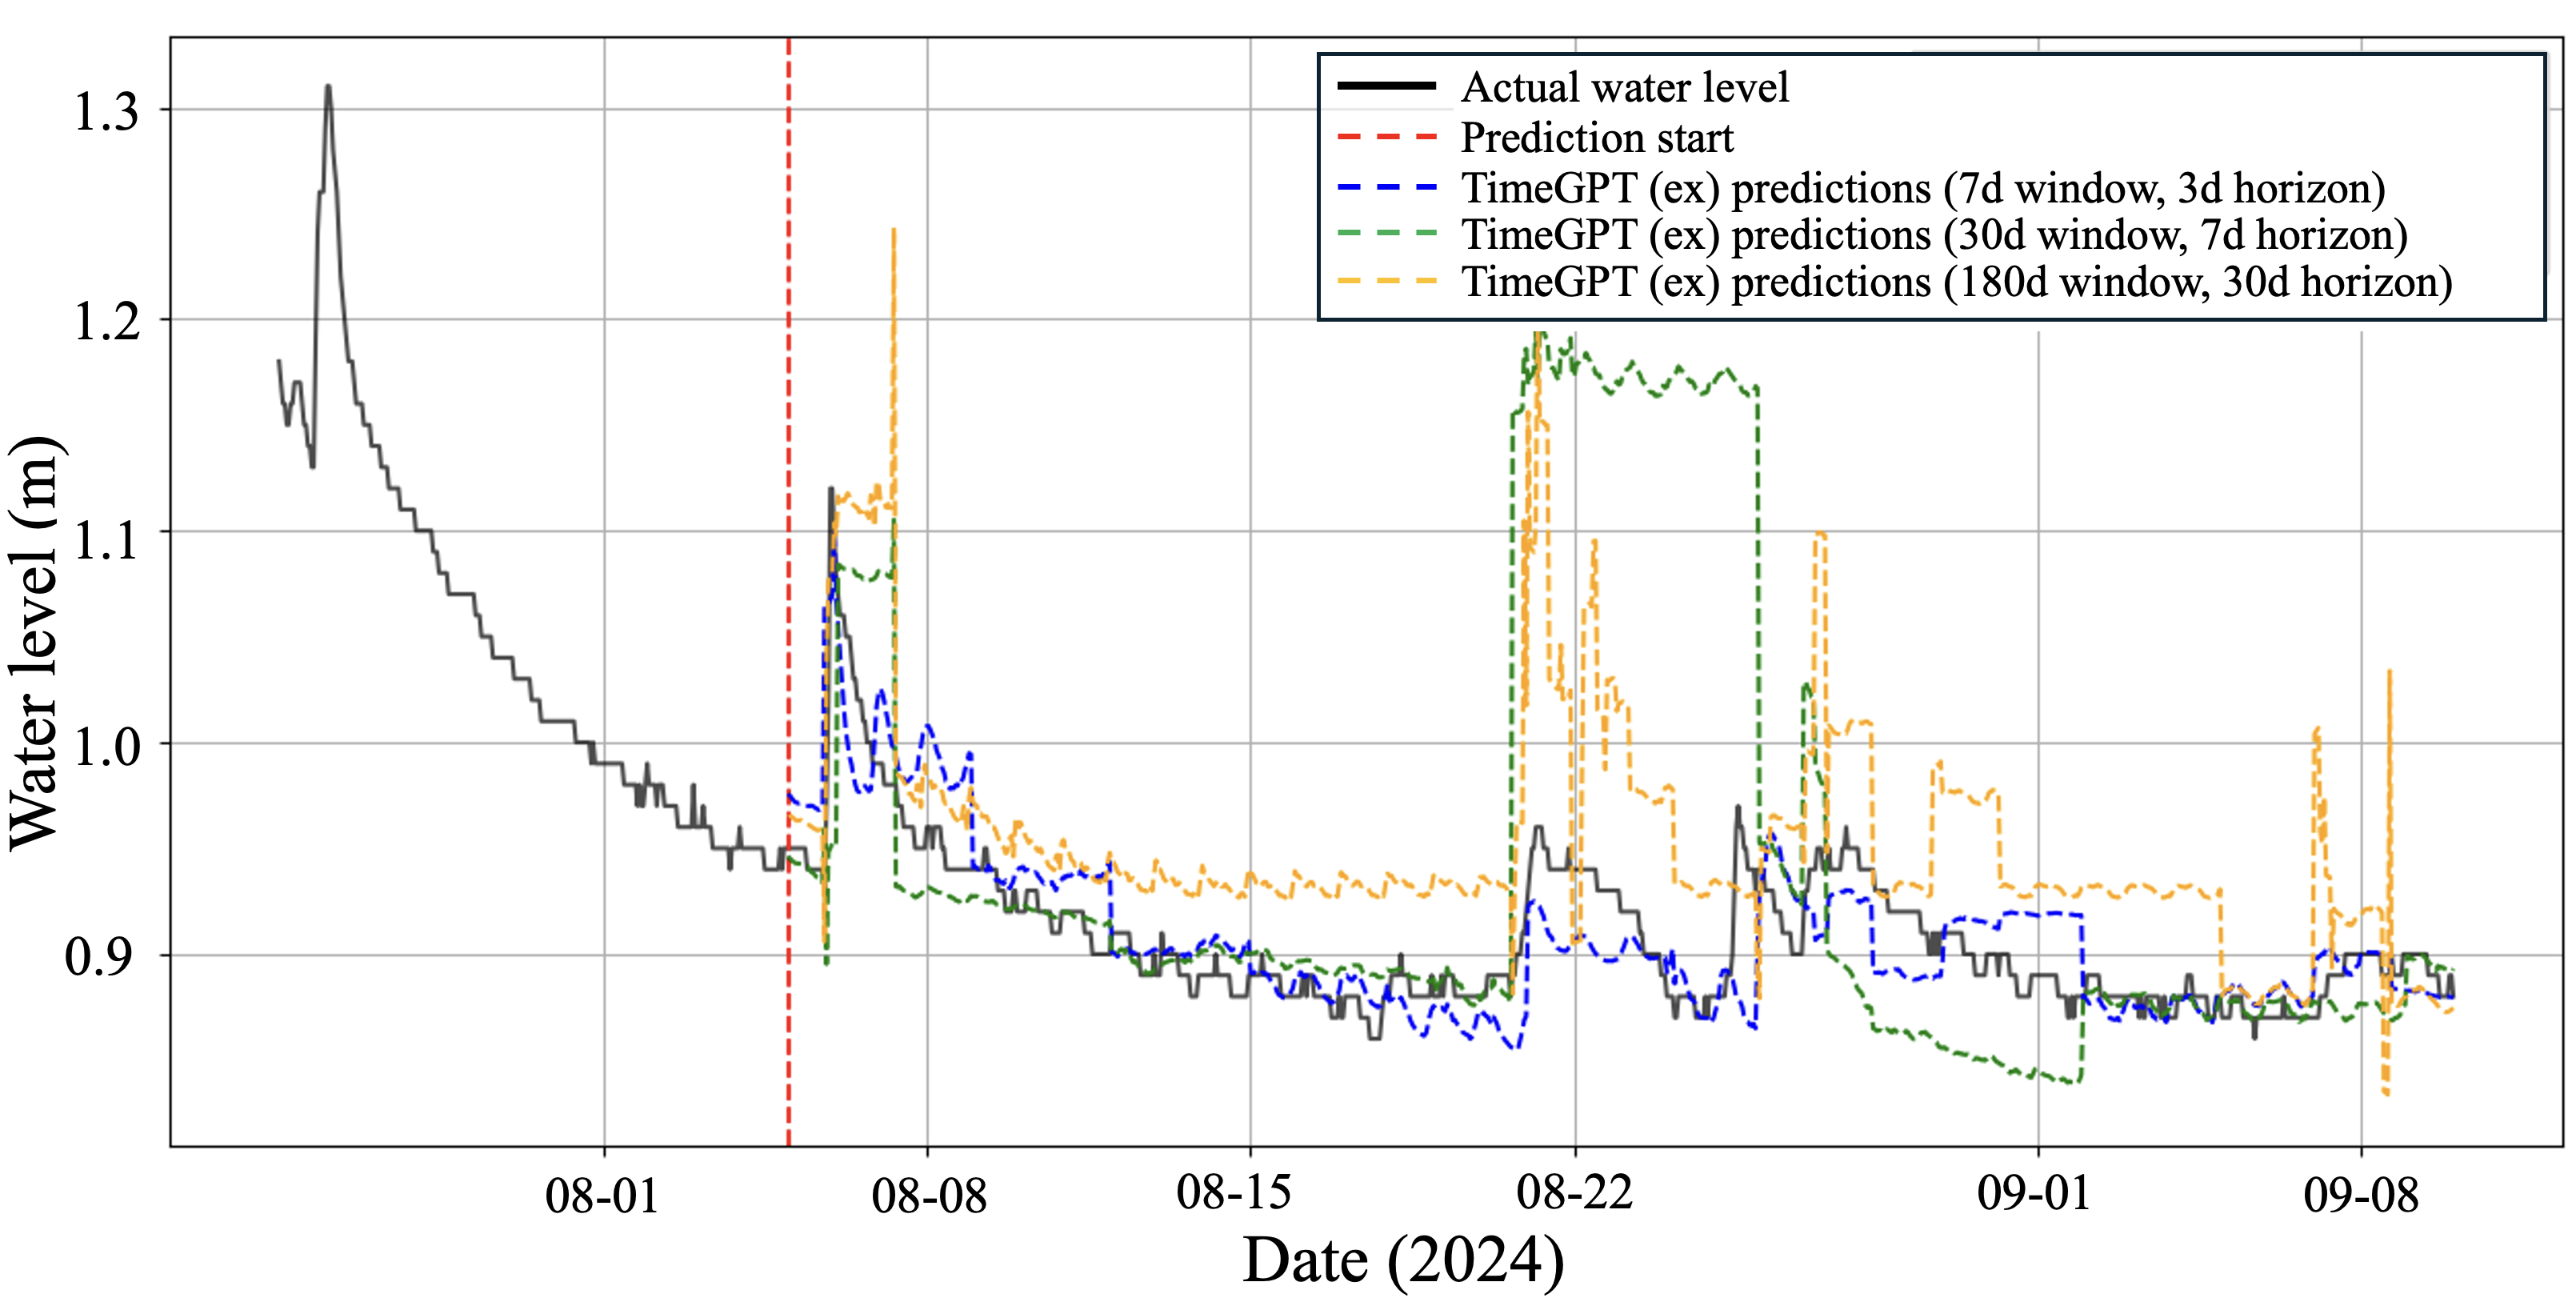
\includegraphics[width=85mm]{TimeGPT_ex_predictions.png}
    \caption{Water level predictions using the TimeGPT (ex) model.}
    \label{fig:time_gpt_predictions_ex}
\end{figure}

Table~\ref{tab:timegpt_comparison_sorted} summarizes the quantitative comparison. For the short-term horizon, TimeGPT~(ex) improves NSE from 0.1360 to 0.5031, while maintaining lower RMSE and MAE across all windows. Even in long-term forecasts ([180,30]), TimeGPT~(ex) achieves an NSE of 0.3369—an order of magnitude higher than the base model’s 0.0138—demonstrating enhanced robustness against non-stationary environmental conditions.

\begin{table}[H]
    \centering
    \caption{Performance comparison of base TimeGPT and TimeGPT (ex).}
    \begin{tabular}{|c|l|c|c|c|}
        \hline
        \rowcolor{gray!20} \textbf{Window} & \textbf{Model} & \textbf{MAE} & \textbf{NSE} & \textbf{RMSE} \\ \hline
        \multirow{2}{*}{{[}7,3{]}} & TimeGPT & 0.0737 & 0.1360 & 0.2067 \\ 
         & TimeGPT (ex) & \textbf{0.0612} & \textbf{0.5031} & \textbf{0.1567} \\ \hline
        \multirow{2}{*}{{[}30,7{]}} & TimeGPT & 0.0897 & 0.1039 & 0.2105 \\ 
         & TimeGPT (ex) & \textbf{0.0889} & \textbf{0.3496} & \textbf{0.1793} \\ \hline
        \multirow{2}{*}{{[}180,30{]}} & TimeGPT & 0.1120 & 0.0138 & 0.2208 \\ 
         & TimeGPT (ex) & \textbf{0.1017} & \textbf{0.3369} & \textbf{0.1810} \\ 
        \hline
    \end{tabular}
    \label{tab:timegpt_comparison_sorted}
\end{table}


Figure~\ref{fig:time_gpt_predictions_overall} and Figure~\ref{fig:time_gpt_predictions_ex_overall} present the overall prediction performance of the base TimeGPT and TimeGPT~(ex) models, respectively.

\begin{figure}[H]
    \centering
    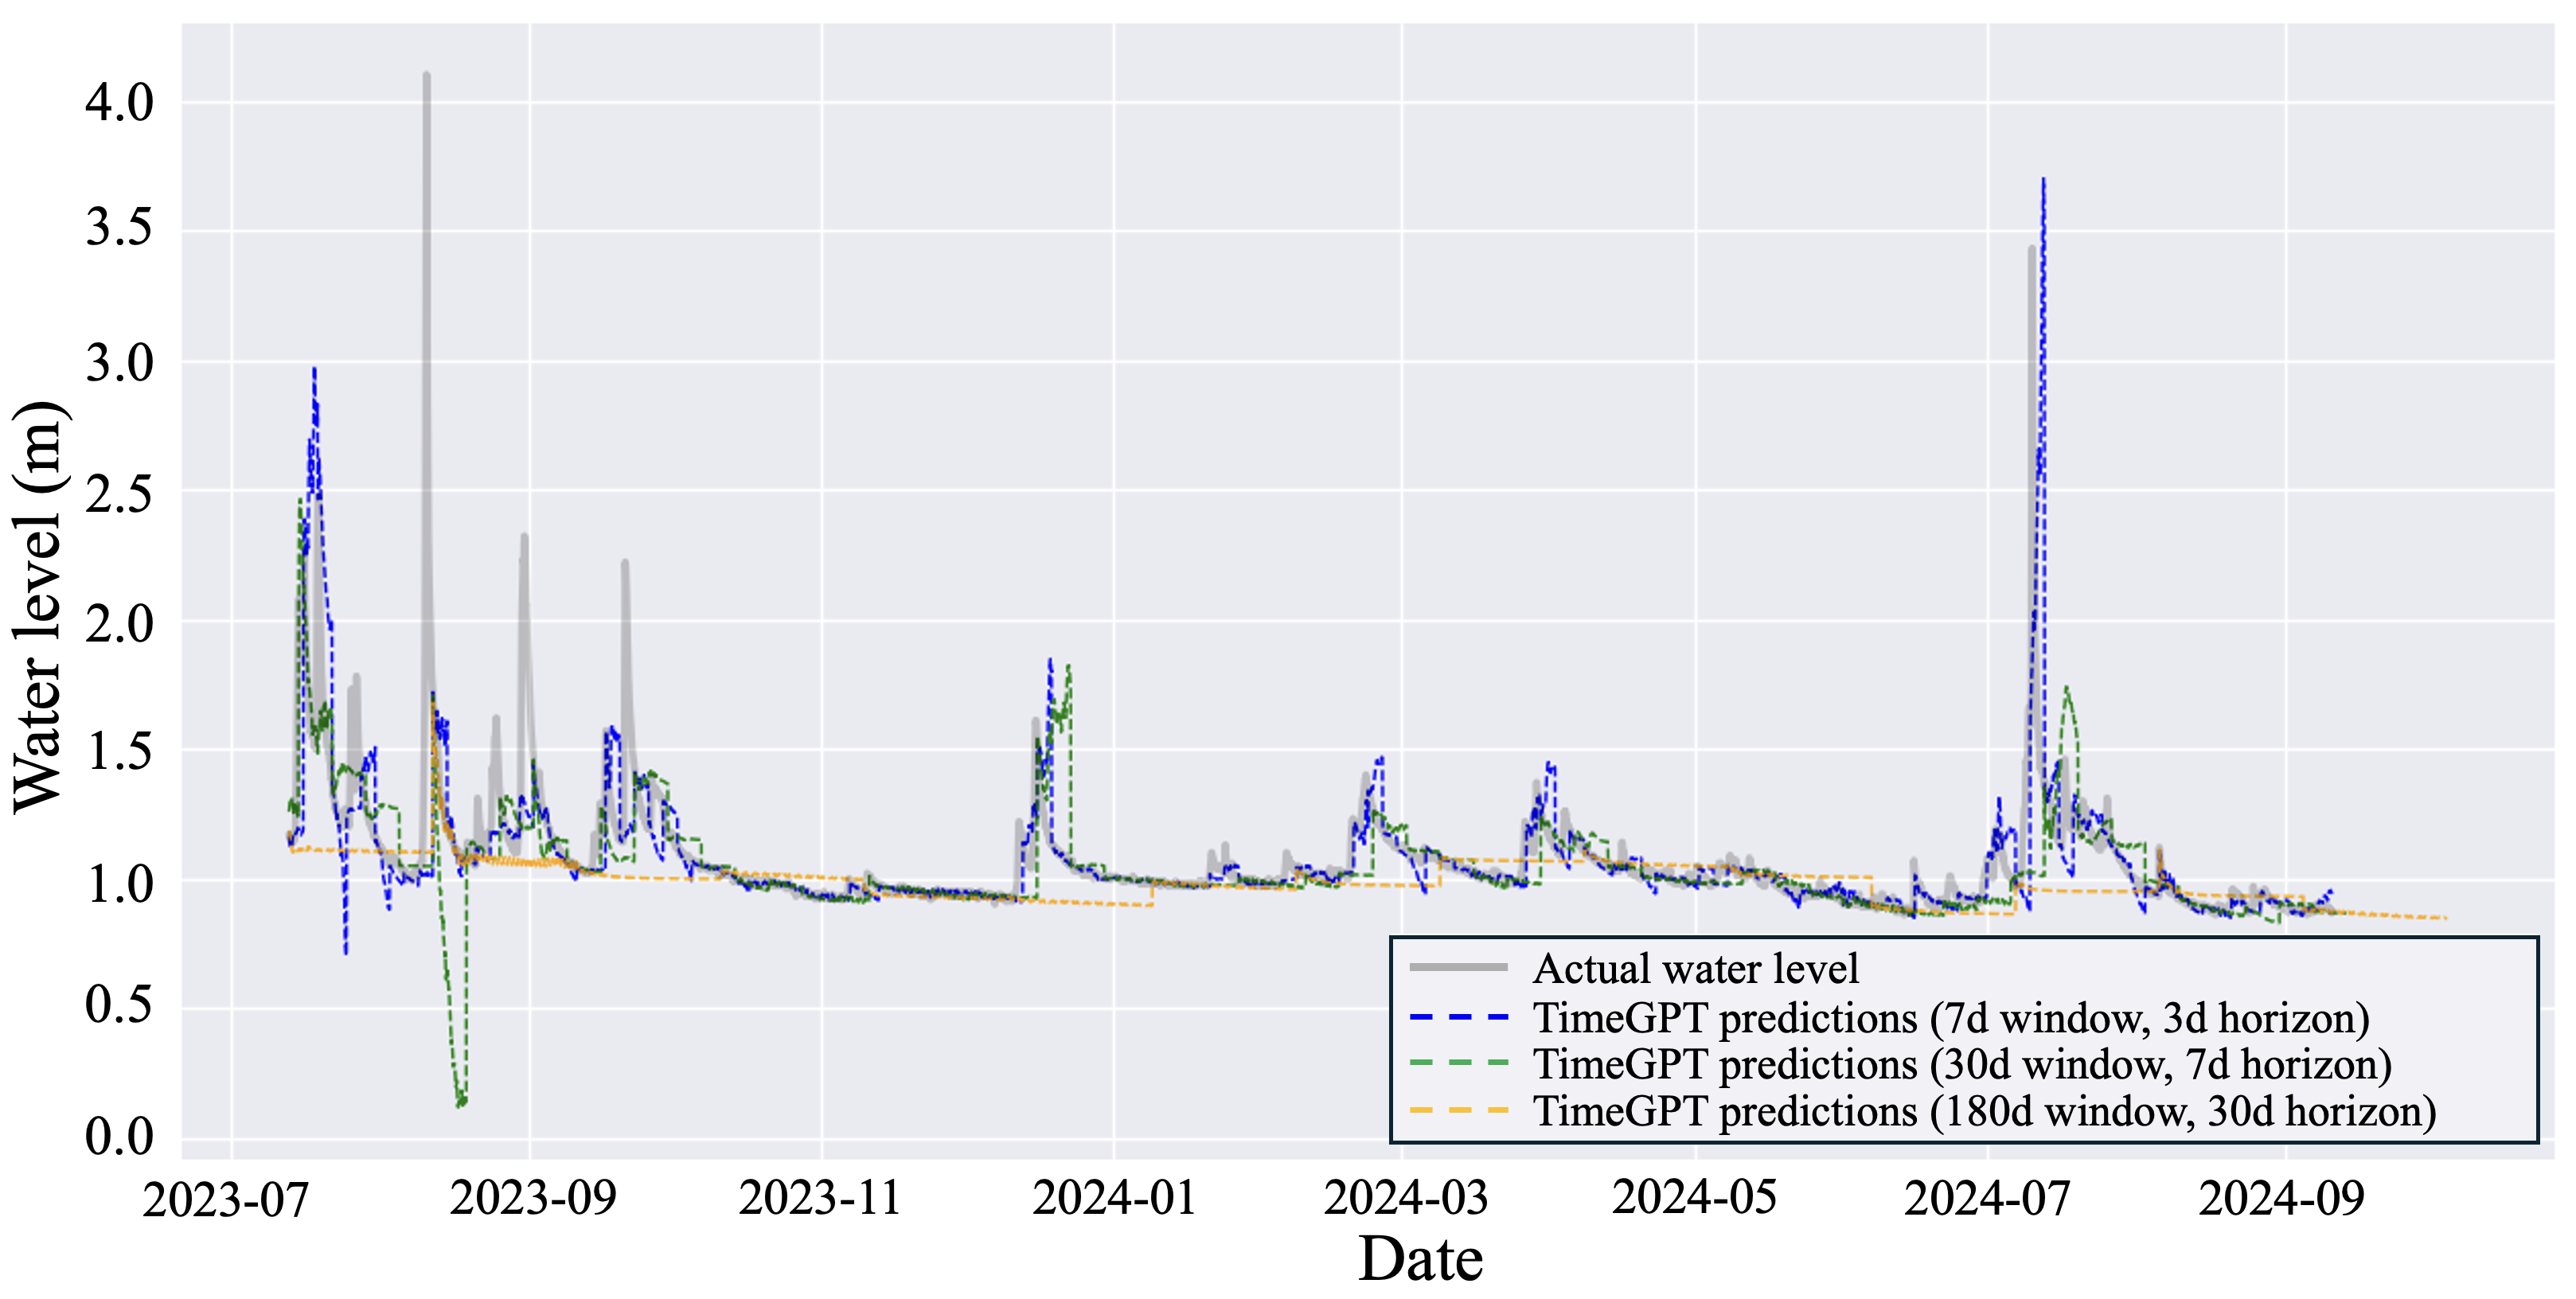
\includegraphics[width=85mm]{TimeGPT_overall.png}
    \caption{Overall performance of the base TimeGPT model.}
    \label{fig:time_gpt_predictions_overall}
\end{figure}

\begin{figure}[H]
    \centering
    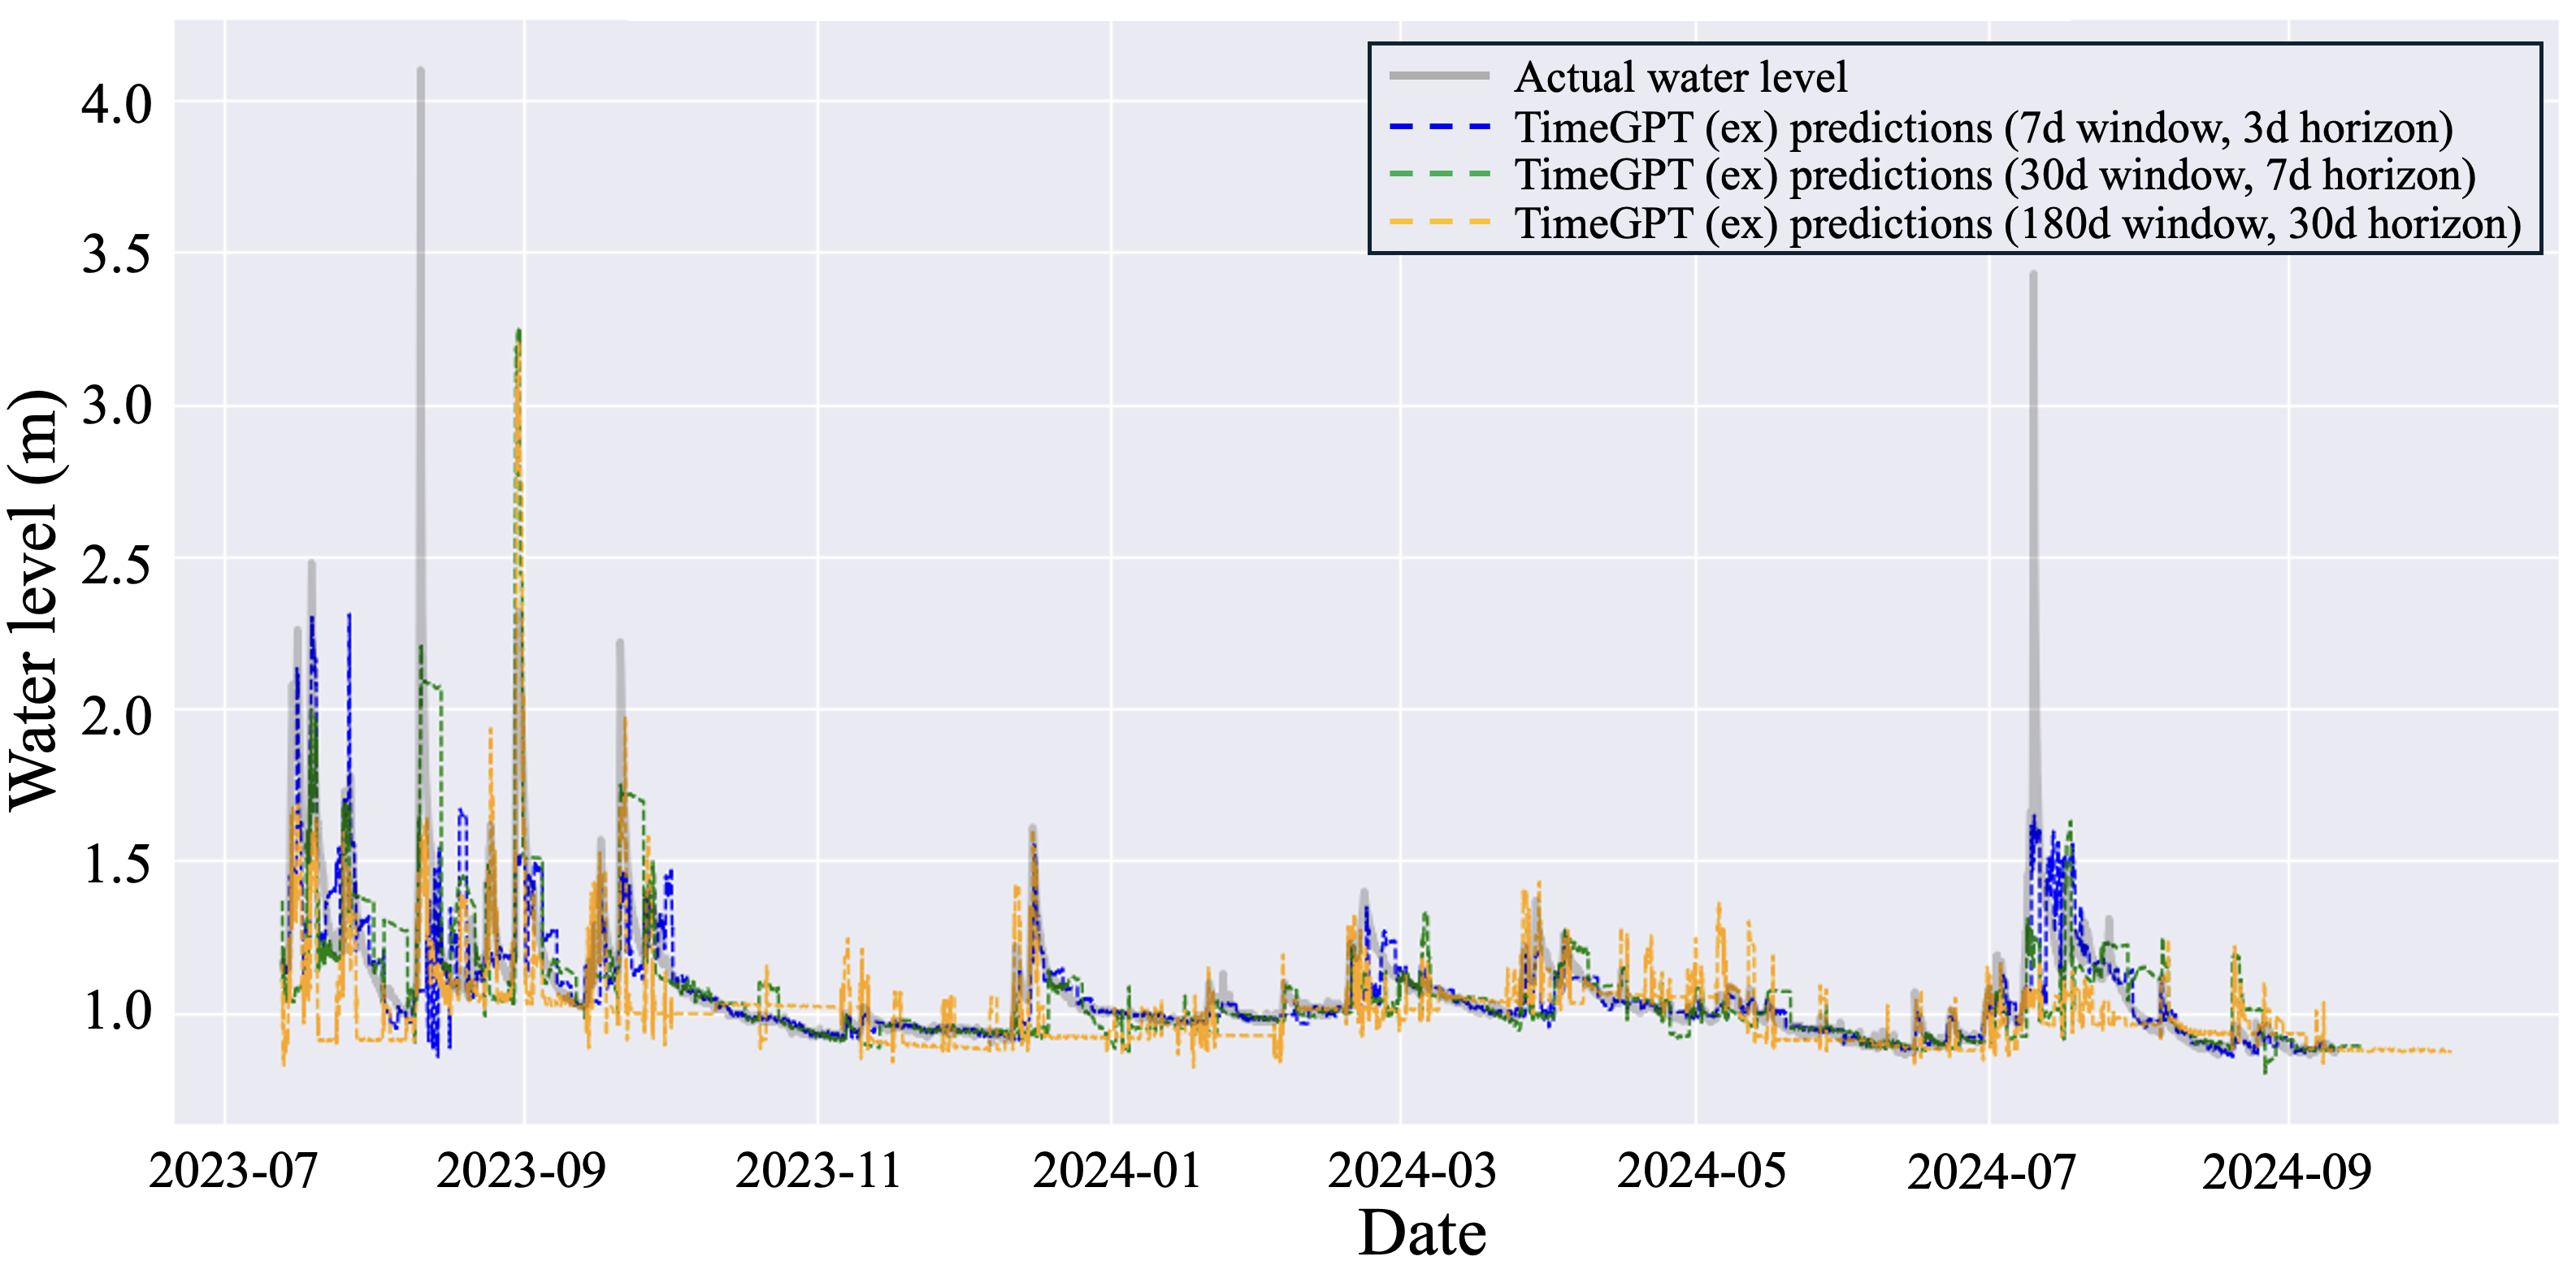
\includegraphics[width=85mm]{TimeGPT_ex_overall.png}
    \caption{Overall performance of the TimeGPT (ex) model.}
    \label{fig:time_gpt_predictions_ex_overall}
\end{figure}

Both models exhibit a pattern common in environmental time series: a gradual decline in predictive accuracy as the forecast horizon lengthens. This trend is evidenced by the progressive increase in RMSE and decrease in NSE scores. For instance, in the base model, the RMSE value increases from 0.2067 for the [7,3] window to 0.2208 for the [180,30] window. However, the figures clearly show that TimeGPT~(ex) consistently maintains higher accuracy across all horizons.

Two primary findings are evident from the results. First, both models exhibit a gradual decline in accuracy as the forecast horizon lengthens, a typical pattern in time-series forecasting. Second, TimeGPT~(ex) consistently outperforms the base model, maintaining higher NSE and lower RMSE values across all forecast horizons.

Beyond the overall performance metrics, specific anomalies are observable in the prediction plots. In August 2023 and July 2024, both models show significant deviations from the observed water levels. These periods are documented to coincide with planned dam releases, which were external interventions not included as input features to the models.



\section{Conclusion}

This study presents three key contributions to water level forecasting for the Gamcheon River. First, we conducted a comprehensive comparison of classical models (ARIMA, SARIMAX), linear models, and LLM-based models. The comparative analysis revealed that while classical models provide stable performance under normal conditions, they show limitations during extreme events. Second, the TimeGPT (ex) model incorporating rainfall data demonstrated significant improvements in forecasting accuracy, with NSE scores increasing from 0.1360 to 0.5031 for short-term predictions and from 0.0138 to 0.3369 for long-term forecasts. These results validate the effectiveness of combining environmental variables with LLM architectures. Third, our scenario-based evaluation methodology confirmed the model's reliability during critical events, such as the September 2024 flood, demonstrating its practical applicability in real-world situations.

The advantages of our proposed approach are multifold. First, it significantly enhances predictive performance in extreme hydrological conditions, providing a more reliable foundation for flood early warning systems. Regarding computational efficiency, while TimeGPT incurs a higher inference latency (~3 seconds) compared to the millisecond-scale inference of Linear models, this cost is negligible for operational hourly forecasting and is well-justified by the substantial gains in accuracy and safety. Second, this study validates the "foundation model hypothesis" in a zero-shot setting, demonstrating that a model trained on global hydrological data can generalize to local catchments without the overfitting risks associated with fine-tuning on limited historical records. Finally, leveraging a pre-trained foundation model presents an efficient alternative to developing complex deep learning models from scratch, allowing for rapid adoption of state-of-the-art AI.

While this study demonstrates the strong generalization ability of TimeGPT, two practical challenges remain. First, the model’s sensitivity to input data quality—such as rain gauge density and update frequency—requires further quantification. Comprehensive sensitivity analysis across different spatial and temporal granularities will be an essential direction for future research. Second, the influence of man-made interventions remains a critical limitation. We identified that sudden water level changes driven by dam releases (e.g., August 2023, July 2024) were difficult to predict using only rainfall-runoff dynamics. Future work will incorporate dam operational metadata (discharge schedules) as explicit exogenous variables, enabling the model to capture the causal link between discharge events and downstream level rises more effectively than traditional statistical approaches.

\medskip
\section*{Conflict of Interest}
\noindent
No potential conflict of interest relevant to this article was reported.

\medskip
\section*{Acknowledgement}
\noindent
This work was supported by Korea Environmental Industry \& Technology Institute (KEITI) through R\&D Program for Research and Development on the Technology for Securing the Water Resouces Stability in Response to Future Change, funded by Korea Ministry of Environment (MOE)(RS-2024-00332494).

\begin{thebibliography}{00}

\bibitem{KCP2023}
S. Kwon, Y. Cha, Y. Park, S. Lee, Assessing the impacts of dam/weir operation on streamflow predictions using LSTM across South Korea, Scientific Reports, vo1. 13, no. 9296, 2023. \href{https://doi.org/10.1038/s41598-023-36439-z}{https://doi.org/10.1038/s41598-023-36439-z}

\bibitem{YY24}
S. Yi., J. Yi, Reservoir‑based flood forecasting and warning: deep learning versus machine learning, Applied Water Science, vol.14, no.237, 2024. \href{https://doi.org/10.1007/s13201-024-02298-w}{https://doi.org/10.1007/s13201-024-02298-w}

\bibitem{VSP17}
A. Vaswani, N. Shazeer, N. Parmar, et al.,
``Attention is all you need,'' \emph{Advances in Neural Information Processing Systems}, Long Beach, CA, vol. 30, pp. 5998--6008, 2017.

\bibitem{XFL23}
J. Xu, H. Fan, and M. Luo, et al.,
``Transformer based water level prediction in Poyang Lake, China,'' \emph{Water}, vol. 15, no. 3, pp. 576, 2023. \href{https://doi.org/10.3390/w15030576}{https://doi.org/10.3390/w15030576}

\bibitem{HS1997}
S. Hochreiter and J. Schmidhuber,
``Long short-term memory,'' \emph{Neural Computation}, vol. 9, no. 8, pp. 1735--1780, 1997. \href{https://doi.org/10.1162/neco.1997.9.8.1735}{https://doi.org/10.1162/neco.1997.9.8.1735}

\bibitem{GS2005}
A. Graves and J. Schmidhuber,
``Framewise phoneme classification with bidirectional LSTM and other neural network architectures,'' \emph{Neural Networks}, vol. 18, no. 5--6, pp. 602--610, 2005. \href{https://doi.org/10.1016/j.neunet.2005.06.042}{https://doi.org/10.1016/j.neunet.2005.06.042}

\bibitem{ZCLX23}
A. Zeng, M. Chen, L. Zhang, and Q. Xu,
``Are Transformers Effective for Time Series Forecasting?'' \emph{Proceedings of the AAAI Conference on Artificial Intelligence}, vol. 37, 2023. Washington DC, February 7–14, 2023, pp. 11121--11128. \href{https://doi.org/10.1609/aaai.v37i9.26317}{https://doi.org/10.1609/aaai.v37i9.26317}

\bibitem{BJ1970}
G. E. P. Box and G. M. Jenkins,
``Time series analysis: Forecasting and control,'' \emph{Holden-Day}, San Francisco, 1970, pp. 553.

\bibitem{BJ2015}
G. E. P. Box, G. M. Jenkins, G. C. Reinsel, and G. M. Ljung,
``Time series analysis: Forecasting and control,'' 5th ed., \emph{John Wiley and Sons}, New Jersey, 2015, pp. 712. \href{ https://doi.org/10.1057/9781137291264\_6}{ https://doi.org/10.1057/9781137291264\_6}

\bibitem{HK2008}
R. J. Hyndman and Y. Khandakar,
``Automatic time series forecasting: The forecast package for R,'' \emph{Journal of Statistical Software}, vol. 27, no. 3, pp. 1--22, 2008. \href{https://doi.org/10.18637/jss.v027.i03}{https://doi.org/10.18637/jss.v027.i03}

\bibitem{TL2018}
S. Taylor and B. Letham,
``Forecasting at scale,'' \emph{American Statistician}, vol. 72, no. 1, pp. 37--45, 2018. \href{https://doi.org/10.1080/00031305.2017.1380080}{https://doi.org/10.1080/00031305.2017.1380080}

\bibitem{JWM2024}
M. Jin, S. Wang, L. Ma, et al.,
``TIME-LLM: Time Series Forecasting by Reprogramming Large Language Models,'' \emph{International Conference on Learning Representations}, Vienna Austria. May 7--11, 2024.

\bibitem{LJX2019}
Y. Li, J. Jin, Z. Xuan, et al.,
``Enhancing the Locality and Breaking the Memory Bottleneck of Transformer on Time Series Forecasting,'' \emph{Advances in Neural Information Processing Systems}, vol. 32, 2019.

\bibitem{ZZP2021}
H. Zhou, S. Zhang, J. Peng, et al.,
``Informer: Beyond Efficient Transformer for Long Sequence Time-Series Forecasting,'' \emph{AAAI Conference on Artificial Intelligence}, vol. 35, no. 12, pp. 11106--11115, February 2--9, 2021.
\href{https://doi.org/10.1609/aaai.v35i12.17325}{https://doi.org/10.1609/aaai.v35i12.17325}

\bibitem{XTZ2021}
S. Xu, Y. Tang, Z. Zhu, et al.,
``Autoformer: Decomposition Transformers with Auto-Correlation for Long-Term Series Forecasting,'' \emph{Advances in Neural Information Processing Systems}, vol. 34, pp. 22419--22430, 2021.

\bibitem{LLZ2021}
D. Liu, W. Lin, W. Zhou, et al.,
``Pyraformer: Low-Complexity Pyramidal Attention for Long-Range Time Series Modeling and Forecasting,'' \emph{International Conference on Learning Representations}, May 3--7, 2021.

\bibitem{ZZ2022}
H. Zhou, S. Zhang, et al.,
``FEDformer: Frequency Enhanced Decomposed Transformer for Long-Term Series Forecasting,'' \emph{Advances in Neural Information Processing Systems}, pp. 27268-27286, 2022.

\bibitem{GM2023}
A. Garza, M. Mergenthaler-Canseco,
``TimeGPT-1,'' \emph{arXiv preprint arXiv:2310.03589}, 2023.

\bibitem{LWY2025}
W. Liao, S. Wang, D. Yang, et al.,
``TimeGPT in load forecasting: A large time series model perspective,'' \emph{Applied Energy}, vol. 379, p. 124973, 2025. \href{https://doi.org/10.1016/j.apenergy.2024.124973}{https://doi.org/10.1016/j.apenergy.2024.124973}

\end{thebibliography}

%=============================
\raggedbottom

\newpage
\parpic[l]{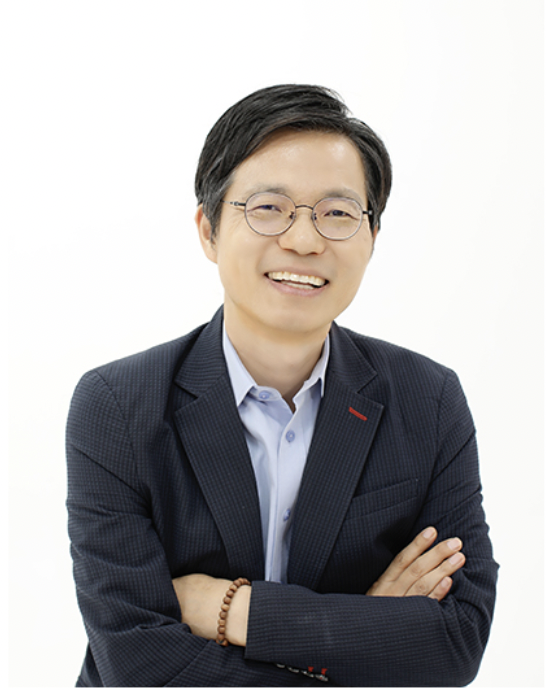
\includegraphics[width=1in,height=1.25in,clip,keepaspectratio]{CA1.jpg}
}
\noindent
{\bf Jon-Lark Kim} received his B.S. degree
in mathematics from Pohang University
of Science and Technology (POSTECH),
finished the master’s course in mathematics from Seoul National University, and
received his Ph.D. in mathematics from
the University of Illinois at Chicago, in 1993, 1997, and 2002,
respectively. He joined the University of Nebraska-Lincoln
from 2002 to 2005 as a research assistant professor. He joined
the University of Louisville between 2005 and 2012 as an assistant and association professor. Since 2012, he has been a
professor at the Department of Mathematics at Sogang University, Seoul, Korea. His research interests include coding theory,
cryptography, soft computing, and artificial intelligence.\\

\parpic[l]{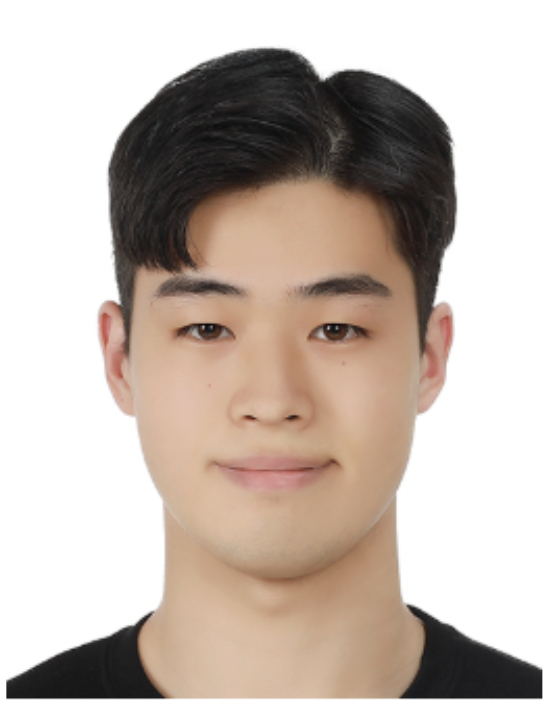
\includegraphics[width=1in,height=1.25in,clip,keepaspectratio]{A1.jpg}
}
\noindent
{\bf Jae-Hyun Baek} received his B.S. degree from Sogang University, Seoul, Korea. He is currently hoping to pursue an M.S. degree in the Department of Mathematics at Sogang University, Seoul, Korea. His research interests include Deep Learning, Image Analysis, large language models (LLMs), and AI security.\\

\parpic[l]{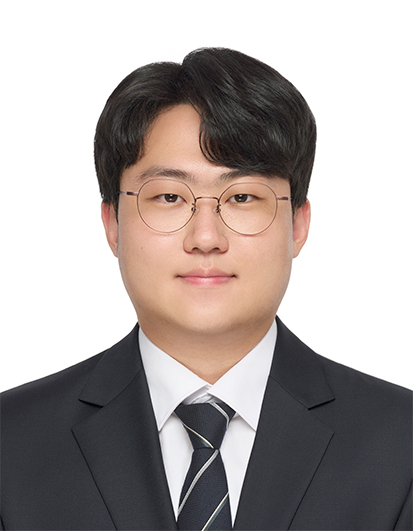
\includegraphics[width=1in,height=1.25in,clip,keepaspectratio]{A2.jpg}
}
\noindent
{\bf Keon-Hwi Kim} received his B.S. degree
in Mathematics from Incheon National
University. He is currently pursuing an
M.S. degree in the Department of Mathematics at Sogang University, Seoul, Korea. His research interests include data
science, focusing on similarity measures,
vector databases, classification, and time series forecasting. He also studied large language models (LLMs) and artificial intelligence.\\
\noindent

\parpic[l]{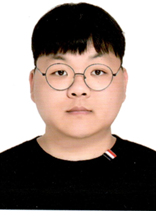
\includegraphics[width=1in,height=1.25in,clip,keepaspectratio]{A3.jpg}
}
\noindent
{\bf Tae Hyo Baek} earned his B.S., M.S., and Ph.D. degrees in Civil Engineering from Korea National University of Transportation, Korea, in 2018, 2020, and 2025, respectively. He has been serving as a postdoctoral researcher in the Department of Civil Engineering at Korea National University of Transportation, Korea. His research interests include river hydraulics, numerical modeling of geomorphic changes, and sediment transport.\\

\parpic[l]{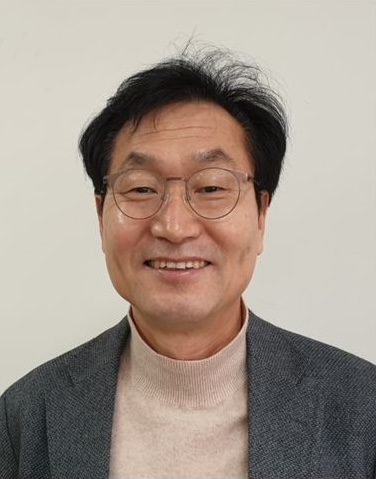
\includegraphics[width=1in,height=1.25in,clip,keepaspectratio]{CA2.jpg}
}
\noindent
{\bf Chang-Lae Jang} earned his B.S. and M.S. degrees in Civil Engineering from Chungnam National University, Korea, in 1993 and 1999, respectively, and his Ph.D. in Civil Engineering from Hokkaido University, Japan, in 2003. From 2004 to 2009, he worked as a senior researcher at the K-water Institute. Since 2009, he has been serving as a professor in the Department of Civil Engineering at Korea National University of Transportation, Korea. His research focuses on sediment transport processes in rivers, fluvial dynamics in vegetated rivers, numerical simulations of river morphology, river meandering and braiding mechanics, and reservoir sedimentation.\\
\noindent

\bigskip
\bigskip
\bigskip
\bigskip
\bigskip
\bigskip
\bigskip
\bigskip
\bigskip
\bigskip
\bigskip
\bigskip
\bigskip

 
\end{document}

\subsection{Submission of Manuscripts}
\noindent

IJFIS receives the papers only through the electronic submission via http://ijfis.org, except for very special circumstances that the IJFIS recognizes. This web site provides the standard submission process in steps. This system will ask the author(s) to upload the PDF or Microsoft Word file(s) of the paper.

Regular papers normally have a length of 10-20 double-spaced pages (counting one figure as 1/3 of a page) of A4 size papers. Longer manuscripts will be considered, but have a proportionately lower probability of acceptance. Each paper must include an abstract of no more than 250 words and a list of no more than five keywords, Regular papers are sent to three experts in the filed for detailed review. Based on the reviews and the recommendation off the responsible editor, the editorial board finalized acceptance or rejection of the paper.




\subsection{Manuscript}
\noindent
Since the IJFIS publishes only in English, contributors for whom English is not a native language should consult a colleague who is familiar with the English language, prior to submitting the paper, for the purpose of editing the original manuscript. All manuscripts should be prepared according to the following guidelines:

 


 


\subsubsection{ TEXT-TYPES OF ARTICLES}

\begin{itemize}


\item The research paper should be presented in a structured format, (1) Introduction, (2) Theory and Methods, (3) Results, (4) Discussion, and (5) Conclusion. This clearly states the problem and the objective of the research, describes the method so it can be duplicated and its validity judged, reports the results accurately and briefly, provides discussion of findings, lists the conclusions that may be drawn from the research, and provides contributions of the work. 

\item The literature review accurately records the sequence of development of a particular phase of dentistry; is brief but also complete; and provide documentation by references.

\item Specify grant or other financial support, citing the name of the supporting organization and grant number.
\end{itemize}


FIGURES

\begin{itemize}


\item All figures must be scanned and saved as an electronic file.

\item The files should be numbered and cited in the text in order of appearance.
\end{itemize}

%++++++++++++++++++++++++++++++++++++++++++++++++++++++++++++++++
\begin{figure}[t]
\centering

\includegraphics[width=70mm]{main1}
\vskip -0.5pc
\caption{Caption for the figure.}
\label{fig:main}
\end{figure}
%+++++++++++++++++++++++++++++++++++++++++++++++++++++++++++++++

TABLES

\begin{itemize}


\item Must include column heads, footnotes, and data. The table should list all abbreviations in the table in footnotes at the end.

\item Should be numbered according to their order of mention in the text. Each table must be submitted as an electronic file. Omit internal horizontal and vertical lines.

\item Should have a title that is concise and describes the table\rq{}s contents. The table should be self-explanatory and supplement, not duplicate the text.

\item If the table or any data therein have been published, a footnote to the table must give full credit to the original source.
\end{itemize}





  
%
\begin{equation}
k\left[(x-C_{x})^2 + (z-C_{z})^2\right] + l(y-C_{y})^2 - r^2 = 0
\label{eq:ell}
\end{equation}
 
%++++++++++++++++++++++++++++++++++++++++++++++++++++++++++++++++
 
%++++++++++++++++++++++++++++++++++++++++++++++++++++++++++++++++
  
%===========================================================
\section{Conclusions}
\noindent
The Conclusions section should be included in the manuscript. 

\medskip
\section*{Conflict of Interest}
\noindent
No potential conflict of interest relevant to this article was reported.


%===========================================================
\bibliographystyle{ieeetr}

\medskip
\begin{thebibliography}{1}
 
\bibitem{ross10} 
 T. ~J. ~Ross, {\it Fuzzy Logic with Engineering Applications}, 3rd ed., Chichester: John Wiley \& Sons, 2010.

\bibitem{zhang111}
 S. ~Zhang, J. Yin, and W. Guo, \lq\lq{}Pool-base active learning with query construction,\rq\rq{} in {\it Foundations of Intelligent Systems}, Y. Yang and T. Li, Eds. Berlin: Springer-Verlag, 2011, pp.13-22. 

\bibitem{kim12}
  Y. ~H. ~Kim, H. Lee, and S. Kim, \lq\lq{}3D radar objects tracking and reflectivity profiling,\rq\rq{} {\it International Journal of Fuzzy Logic and Intelligent Systems}, vol. 12, no. 4, pp. 263-269, Dec. 2012. \url{http://dx.doi.org/ 10.5391/IJFIS.2012.12.4.263}

\bibitem{montalvo12}
 S. ~Montalvo, E. ~G. ~Pardo, R. Martinez, and V. ~Fresno, \lq\lq{}Automatic cognate identification based on a fuzzy combination of string similarity measures,\rq\rq{} in {\it Proceedings of 2012 IEEE International Conference on Fuzzy Systems}, Brisbane, 2012, pp.1-8. \url{ http://dx.doi.org/10.1109/FUZZ-IEEE.2012.6250802}

\bibitem{arrillaga90}
  J. ~Arrillaga and B. ~Giessner, \lq\lq{}Limitation of short-circuit levels by means of HVDC links,\rq\rq{} presented at {\it the IEEE Summer Power Meeting}, Los Angeles, CA, July 12–17, 1990, Paper 70 CP 637.

\bibitem{de06}
  A. ~De, \lq\lq{}Fuzzy result merging models for metasearch,\rq\rq{}  Ph.D. dissertation, Department of Computer Science, University of Louisiana at Lafayette, Lafayette, LA, 2006.

\bibitem{kim09}
 J. ~C. ~Kim, \lq\lq{}ocal path planning algorithm based on candidate trajectory optimization,\rq\rq{} M.S. thesis, Korea Advanced Institute of Science and Technology, Daejeon, Korea, 2009.



\end{thebibliography}